%------------------------------------------------------------------------------
% Copyright (c) !!COPYRIGHTYEAR!!, Xavier Leroy and Didier Remy.  
%
% All rights reserved. Distributed under a creative commons
% attribution-non-commercial-share alike 2.0 France license.
% http://creativecommons.org/licenses/by-nc-sa/2.0/fr/
%
% Translation by Richard Paradies
%------------------------------------------------------------------------------

\chapter{Files}
\label{sec/files}
\cutname{files.html}

The term \quotes{file} in Unix covers several types of objects:
%
\begin{itemize}
\item standard files: finite sets of bytes containing text or binary
  information. We may call them \quotes{ordinary} files.
%
\item directories.
%
\item symbolic links.
%
\item special files (\emph{devices}), which give, in particular, access
  to computer peripherals.
%
\item named pipes.
%
\item sockets named in the Unix domain.
\end{itemize}
% 
The file concept includes both the data contained in the file and
information about the file itself (also called meta-data) like its
type, its access privileges, the latest access dates, {\etc}

\section{The file system}

As a first approximation, the file system is as a tree. The root is
represented by \ml+'/'+ . The branches are labeled by (file) names,
which are strings of any characters excluding \ml+'\000'+ and \ml+'/'+
(but it is good practice to also avoid non-printing characters and
spaces). The non-terminal nodes are \emph{directories}: these nodes
always contain two branches \ml+.+ and {..} which respectively
represent the directory itself and the directory's parent. The other
nodes are sometimes called \emph{files}, as opposed to directories,
but this is ambiguous, as we can also designate any node as a
\quotes{file}. To avoid all ambiguity we refer to them as
\emph{non-directory files}.

The nodes of the file system are addressed by paths. If the root of
the path is the top of the file hierarchy, the path is absolute and if
it is a directory (usually the current working directory) it is
relative. More precisely a \emph{relative path} is a string of file
names separated by the the character \ml+'/'+.  An \emph{absolute
  path} is a relative path preceded by the the character \ml+'/'+
(note the double use of this character both as a separator and as
the name of the root node).

The \libmodule{Filename} module handles file paths in a portable
manner. Notably \libvalue{Filename}{concat} concatenates paths without
using the character \ml+'/'+, allowing the code to function equally
well on other architectures (for example the path separator character
under Windows is \ml+'\'+).  Similarly, the \ml+Filename+ module
provides the string values \libvalue{Filename}{current\_dir\_name} and
\libvalue{Filename}{parent\_dir\_name} to represent the branches
\ml+.+ and \ml+..+ The functions \libvalue{Filename}{basename} and
\libvalue{Filename}{dirname} return the prefix \ml+d+ and the suffix
\ml+b+ from a file path \ml+p+ such that the file path \ml+p+ and
\ml+d/b+ refer to the same file, where \ml+d+ is the directory in
which the file is found and \ml+b+ is the name of the file. The
functions defined in \ml+Filename+ operate only on paths,
independently of their actual existence within the file hierarchy.

In fact, strictly speaking, the file hierarchy is not a tree. First
the directories \ml+.+ and \ml+..+ allow a directory to refer to
itself and to move up in the hierarchy to define paths leading from a
directory to itself. Moreover, non-directory files can have many
parents (we say that they have many \emph{hard links}). Finally,
there are also \emph{symbolic links} which can be seen as
non-directory files containing a path. Conceptually this path can be
obtained by reading the contents of the symbolic link like an ordinary
file. Whenever a symbolic link occurs in the middle of a path we have
to follow its path transparently. If \ml+s+ is a symbolic link whose
value is the path \ml+l+, then the path \ml+p/s/q+ represents the file
\ml+l/q+ if \ml+l+ is an absolute path or the file \ml+p/l/q+ if
\ml+l+ is a relative path.

Figure~\ref{fig/hierarchy} gives an example of a file hierarchy.  The
symbolic link \ml+11+ corresponding to the path \ml+/tmp/bar+ whose
path value is the relative path \ml+./gnu+, does not refer to any
existing file in the hierarchy (at the moment).

\begin{myfigure}
\begin{myimage}[width="100\%"]
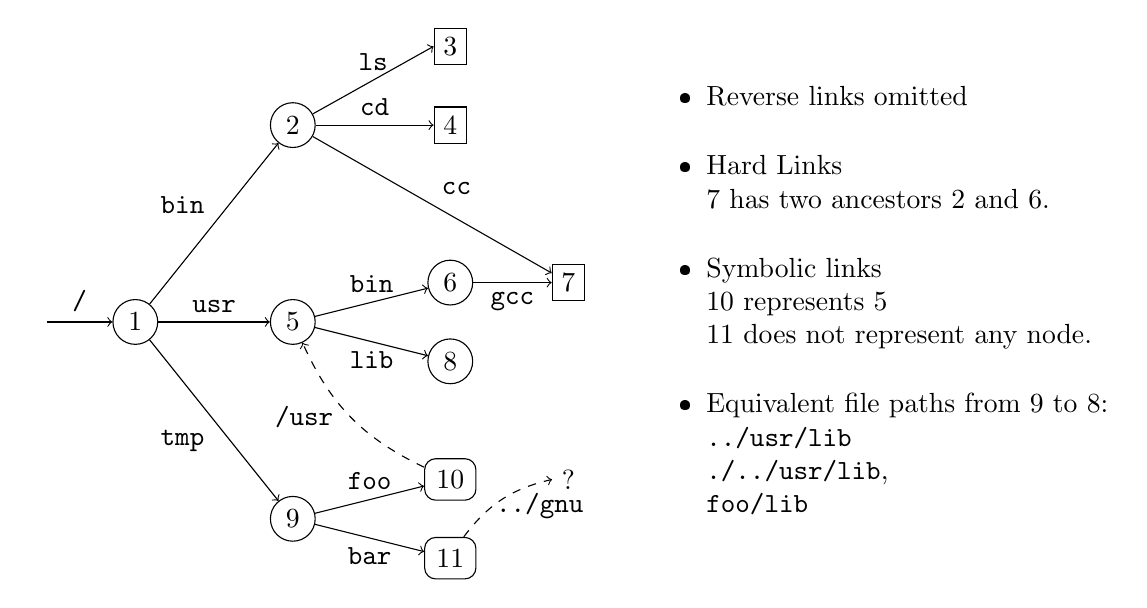
\begin{tikzpicture}
[dir/.style={draw, circle, inner sep=1mm},
 slink/.style={draw,rectangle,inner sep=1.5mm, rounded corners},
 file/.style={draw,rectangle},
 tpath/.style={font={\ttfamily},midway}]
\node (start) at (-1.25,0) {};
\node (n1) at (0,0) [dir] {1};

\node (n2) at (2,2.5) [dir] {2};
\node (n5) at (2,0) [dir] {5};
\node (n9) at (2,-2.5) [dir] {9};

\node (n3) at (4,3.5) [file] {3};
\node (n4) at (4,2.5) [file] {4};
\node (n6) at (4,0.5) [dir] {6};
\node (n8) at (4,-0.5) [dir] {8};
\node (n10) at (4, -2) [slink] {10};
\node (n11) at (4, -3) [slink] {11};

\node (n7) at (5.5, 0.5) [file] {7};
\node (nqmark) at (5.5, -2) {?};

\draw[->] (start) to node [tpath,above] {/} (n1);

\draw[->] (n1) to node [tpath,above left] {bin} (n2);
\draw[->] (n1) to node [tpath,above] {usr} (n5);
\draw[->] (n1) to node [tpath,below left] {tmp} (n9);

\draw[->] (n2) to node [tpath,above] {ls} (n3.west);
\draw[->] (n2) to node [tpath,above] {cd} (n4);
\draw[->] (n2) to node [tpath,above right] {cc} (n7);

\draw[->] (n5) to node [tpath,above] {bin} (n6);
\draw[->] (n5) to node [tpath,below] {lib} (n8);

\draw[->] (n9) to node [tpath,above] {foo} (n10);
\draw[->] (n9) to node [tpath,below] {bar} (n11);

\draw[->] (n6) to node [tpath,below] {gcc} (n7);

\draw[->,dashed] (n10) to [bend left=20] node [tpath,left=1mm] {/usr} (n5);
\draw[->,dashed] (n11) to [bend left=20] node [tpath,below right=-2mm] {../gnu} (nqmark.west);
\node[right=0.75cm, text width=6cm] at (n7)
{
  \begin{itemize}
    \item Reverse links omitted \vspace{5pt}
    \item Hard Links \\ 
      7 has two ancestors 2 and 6.\vspace{5pt}
    \item Symbolic links \\ 
      10 represents 5 \\ 
      11 does not represent any node. \vspace{5pt}
    \item Equivalent file paths from  9 to 8: \\
      \texttt{../usr/lib} \\
      \texttt{./../usr/lib}, {\etc} \\
      \texttt{foo/lib}
  \end{itemize}
};
\end{tikzpicture}
\end{myimage}
\caption{An example of a file hierarchy}
\label{fig/hierarchy}
\end{myfigure}

In general, a recursive traversal of the hierarchy will terminate
if the following rules are respected:
%
\begin{itemize}
\item the directories \ml+.+ and \ml+..+ are ignored.
\item symbolic links are not followed. 
\end{itemize}
% 
But if symbolic links are followed we are traversing a graph and
we need to keep track of the nodes we already visited to avoid loops.

Each process has a current working directory. It is returned by the
function \indexlibvalue{Unix}{getcwd} and can be changed with
\indexlibvalue{Unix}{chdir}.  It is also possible to constrict the
view of the file hierarchy by calling 
\indexlibvalue{Unix}{chroot} \ml+p+. This makes the node \ml+p+, which 
should be a directory, the root of the restricted view of the
hierarchy. Absolute file paths are then
interpreted according to this new root \ml+p+ (and of course \ml+..+ at the
new root is \ml+p+ itself).

\section{File names, file descriptors}

There are two ways to access a file.  The first is by its \emph{file
  name} (or \emph{path name}) in the file system hierarchy.  Due to
hard links, a file can have many different names.  Names are
represented by strings (type \ml+string+). For example the
system calls \syscall{unlink}, \syscall{link}, \syscall{symlink} and
\syscall{rename} all operate at the file name level.
%
\begin{listingcodefile}{tmpunix.mli}
val $\libvalue{Unix}{unlink}$ : string -> unit
val $\libvalue{Unix}{link}$ : string -> string -> unit
val $\libvalue{Unix}{symlink}$ : string -> string -> unit
val $\libvalue{Unix}{rename}$ : string -> string -> unit
\end{listingcodefile}
% 
The call \ml+unlink f+ erases the file \ml+f+ (like the Unix command
\ml+rm -f f+), \ml+link f1 f2+ creates a hard link named \ml+f2+ to
the file \ml+f1+ (like the command \ml+ln f1 f2+), 
\ml+symlink f1 f2+ creates a symbolic link named \ml+f2+ to the file 
\ml+f1+ (like the command \ml+ln -s f1 f2+) and
\ml+rename f1 f2+ renames the file \ml+f1+ to \ml+f2+ 
(like the command \ml+mv f1 f2+).

The other way of accessing a file is by a file descriptor. A
descriptor represents a pointer to a file along with other
information like the current read/write position in the file, the
permissions of the file (is it possible to read ? write ?) and flags
which control the behavior of reads (blocking, non-blocking, \etc) and
writes (overwrite, append, \etc). File descriptors are represented by
values of the abstract type \libtype{Unix}{file\_descr}.

Access to a file via its descriptor is largely independent from the
access via its name. In particular whenever we get a file descriptor,
the file can be destroyed and renamed but the descriptor still points
on the original file.

When a program is executed, three descriptors are allocated and 
tied to the variables \ml+stdin+, \ml+stdout+ and \ml+stderr+ of the
\ml+Unix+ module:
\begin{codefile}{tmpunix.mli}
type file_descr
\end{codefile}
\begin{listingcodefile}{tmpunix.mli}
val $\indexlibvalue{Unix}{stdin}$ : file_descr
val $\indexlibvalue{Unix}{stdout}$ : file_descr
val $\indexlibvalue{Unix}{stderr}$ : file_descr
\end{listingcodefile}
They correspond, respectively, to the standard input, standard output
and standard error of the process.

When a program is executed on the command line without any
redirections, the three descriptors refer to the terminal.  But if,
for example, the input has been redirected using the notation 
\ml+cmd < f+, then the descriptor \ml+stdin+ refers to the file named \ml+f+
during the execution of the command \ml+cmd+. Similarly, \ml +cmd > f+
and \ml+cmd 2> f+ respectively bind the descriptors \ml+stdout+ and
\ml+stderr+ to the file named \ml+f+ during the execution of the
command \ml+cmd+.


\section{Meta-attributes, types and permissions}

The system calls \syscall{stat}, \syscall{lstat} and \syscall{fstat}
return the meta-attributes of a file. This is to say information about
the node itself rather than its content. Among other things, this
information contains the identity of the file, the type of file, the
access rights, the time and date of last access and other additional
information.
%
\begin{codefile}{tmpunix.mli}
type stats
\end{codefile}
%
\begin{listingcodefile}{tmpunix.mli}
val $\libvalue{Unix}{stat}$  : string -> stats
val $\libvalue{Unix}{lstat}$ : string -> stats
val $\libvalue{Unix}{fstat}$ : file_descr -> stats
\end{listingcodefile}
% 
The system calls \ml+stat+ and \ml+lstat+ take a file name as an
argument.  The call \ml+fstat+ takes as an argument a previously
opened descriptor and returns information about the file it points on.
The difference between \ml+stat+ and \ml+lstat+ can be seen on
symbolic links : \ml+lstat+ returns information about the symbolic
link itself , while \ml+stat+ returns information about the file that
the link refers to. The result of these three calls is a record
of type \libtype{Unix}{stats} described in the table~\ref{fig/stats}.
%
\begin{mytable}
\begin{tabular}{lp{9cm}}
Field name & Description \\
%
\hline
\ml+st_dev : int+ 
& The id of the device on which the file is stored. \\
%
\ml+st_ino : int+ 
& The id of the file (inode number) in its partition. 
The pair \ml+(st_dev, st_ino)+ uniquely identifies the file
within the file system. \\
%
\ml+st_kind : file_kind+ & 
The file type. The type \libtype{Unix}{file\_kind} is an enumerated type
whose constructors are:  
\begin{mltypecases}
\begin{tabular}{@{}ll}
\ml+S_REG+ & regular file \\
\ml+S_DIR+ & directory \\
\ml+S_CHR+ & character device  \\
\ml+S_BLK+ & block device  \\
\ml+S_LNK+ & symbolic link \\
\ml+S_FIFO+ & named pipe \\
\ml+S_SOCK+ & socket 
\end{tabular}
\end{mltypecases}
\\
%
\ml+st_perm : int+ & Access rights for the file \\
%
\ml+st_nlink : int+ 
& For a directory: the number of entries in the directory. For others:
the number of hard links on this file. \\
%
\ml+st_uid : int+ & The id of the file's user owner. \\
%
\ml+st_gid : int+ & The id of the file's group owner. \\
%
\ml+st_rdev : int+ 
& The id of the associated peripheral (for special files). \\
%
\ml+st_size : int+ & The file size, in bytes. \\
%
\ml+st_atime : int+ & Last file content access date (In seconds from
January 1st 1970, midnight). \\
%
\ml+st_mtime : int+ & Last file content modification date (Idem).\\
%
\ml+st_ctime : int+ & Last file state modification date: either a
write in the file or a change in access rights, user or group owner,
or number of links.
\smallskip\\
\hline
\end{tabular}
\caption{Fields of the \ml+stats+ structure}
\label{fig/stats}
\end{mytable}

\subsection*{Identification}

A file is uniquely identified by the pair made of its device number
(typically the disk partition where it is located) \ml+st_dev+ and its
inode number \ml+st_ino+.

\subsection*{Owners}

A file has one user owner \ml+st_uid+ and one group owner
\ml+st_gid+.  All the users and groups 
on the machine are usually described in the  
 \ml+/etc/passwd+ and \ml+/etc/groups+ files. We can lookup them by
name in a portable manner with the functions \syscall{getpwnam} and 
\syscall{getgrnam} or by id with 
\syscall{getpwuid} and \syscall{getgrgid}.
%
\begin{codefile}{tmpunix.mli}
type passwd_entry = Unix.passwd_entry
type group_entry = Unix.group_entry
\end{codefile}
%
\begin{listingcodefile}{tmpunix.mli}
val $\libvalue{Unix}{getpwnam}$ : string -> passwd_entry
val $\libvalue{Unix}{getgrnam}$ : string -> group_entry
val $\libvalue{Unix}{getpwuid}$ : int -> passwd_entry
val $\libvalue{Unix}{getgrgid}$ : int -> group_entry
\end{listingcodefile}

The name of the user of a running process and all the groups
to which it belongs can be retrieved with the commands
\syscall{getlogin} and \syscall{getgroups}.
%
\begin{listingcodefile}{tmpunix.mli}
val $\libvalue{Unix}{getlogin}$ : unit -> string
val $\libvalue{Unix}{getgroups}$ : unit -> int array
\end{listingcodefile}

The call \syscall{chown} changes the owner (second argument) and the
group (third argument) of a file (first argument). If we have a file
descriptor, \syscall{fchown} can be used instead. Only the super user
can change this information arbitrarily.
%
\begin{listingcodefile}{tmpunix.mli}
val $\libvalue{Unix}{chown}$ : string -> int -> int -> unit
val $\libvalue{Unix}{fchown}$ : file_descr -> int -> int -> unit
\end{listingcodefile}

%% Le changement de groupe peut se faire sans privil�ge lorsque le
%% programme � un \ml+uid+ (effectif) �gal � celui du fichier et un
%% \ml+gid+ (effectif) �gal au group d�sir� ou � un de ses groupes
%% suppl�mentaire

\subsection*{Access rights}

Access rights are encoded as bits in an integer. The type 
\libtype{Unix}{file\_perm} is just an abreviation for the type
\ml+int+. Access rights specify special bits and read, write and
execution rights for the user owner, the group owner and the other users. 
Access right are thus represented by a vector of bits:
%
\ifhtmlelse{%
\begin{center}
\begin{tabular}{ccc|ccc|ccc|ccc}
\multicolumn{3}{c}{\texttt{S}pecial}
&\multicolumn{3}{c}{\texttt{U}ser}
&\multicolumn{3}{c}{\texttt{G}roup}
&\multicolumn{3}{c}{\texttt{O}ther} \\
\hline
--&--&--&--&--&--&--&--&--&--&--&--\\
\hline
\multicolumn{12}{c}{\ml+OoSUGO+}
\end{tabular}
\end{center}
}
{%
\begin{displaymath}
\underbrace
{\overbrace{---}^{\texttt Special}
 \overbrace{---}^{\texttt User}
 \overbrace{---}^{\texttt Group}
 \overbrace{---}^{\texttt Other}}_{\texttt{0oSUGO}}
\end{displaymath}
}
% 
where in each of the user, group and other fields, the order of bits
indicates read (\ml+r+), write (\ml+w+) and execute (\ml+x+) rights.
The permissions on a file are the union of all these individual
rights, see table~\ref{tab/permbits}.

\begin{mytable}
\begin{tabular}{lcl}
Bit (octal) & Notation \ml+ls -l+ & Right \\
\hline
\ml+0o100+ & \ml+--x------+ & executable by the user owner \\
\ml+0o200+ & \ml+-w-------+ & writable by the user owner \\
\ml+0o400+ & \ml+r--------+ & readable by the user owner \\
\hline
\ml+0o10+  & \ml+-----x---+ &
        executable by members of the group owner. \\
\ml+0o20+  & \ml+----w----+ &
        writable by members of the group owner. \\
\ml+0o40+  & \ml+---r----+ &
        readable by members of the group owner. \\
\hline
\ml+0o1+   & \ml+--------x+ & executable by other users\\
\ml+0o2+   & \ml+-------w-+ & writable by other users \\
\ml+0o4+   & \ml+------r--+ & readable by other users \\
\hline
\ml+0o1000+ & \ml+--------t+ & the bit \ml+t+ on the group (sticky bit)\\
\ml+0o2000+ & \ml+-----s---+ & the bit \ml+s+ on the group (\ml+set-gid+)\\
\ml+0o4000+ & \ml+--s------+ & the bit \ml+s+ on the user (\ml+set-uid+)\\
\hline
\end{tabular}
\caption{Permission bits}\label{tab/permbits}
\end{mytable}

For files, the meaning of read, write and execute permissions is
obvious. For a directory, the execute permission means the right to
enter it (to \ml+chdir+ to it) and read permission the right to list
its contents. Read permission on a directory is however not needed to
read its files or sub-directories (but we then need to know their
names).

The special bits do not have meaning unless the \ml+x+ bit is set (if
present without \ml+x+ set, they do not give additional rights).  This
is why their representation is superimposed on the bit \ml+x+ and
the letters \ml+S+ and \ml+T+ are used instead of \ml+s+ and \ml+t+
whenever \ml+x+ is not set. The bit \ml+t+ allows sub-directories to
inherit the permissions of the parent directory. On a directory, 
the bit \ml+s+ allows to use the directory's \ml+uid+ or \ml+gid+ rather
than the user's one to create directories. For an executable file, 
the bit \ml+s+ allows to change at execution time the user's
effective identity (\syscall{setuid}) or group (\syscall{setgid}).
%
\begin{listingcodefile}{tmpunix.mli}
val $\libvalue{Unix}{setuid}$ : int -> unit
val $\libvalue{Unix}{setgid}$ : int -> unit
\end{listingcodefile}
%
The process also preserves its original identities unless 
it has super user privileges, in which case \ml+setuid+ and
\ml+setgid+ change both its effective and original user and group
identities. The original identity is preserved to allow 
the process to subsequently recover it as its effective identity
without needing further privileges. The system calls \syscall{getuid} and 
\syscall{getgid} return the original identities and 
\syscall{geteuid} and \syscall{getegid} return the effective identities.
%
\begin{listingcodefile}{tmpunix.mli}
val $\libvalue{Unix}{getuid}$ : unit -> int
val $\libvalue{Unix}{geteuid}$ : unit -> int
val $\libvalue{Unix}{getgid}$ : unit -> int
val $\libvalue{Unix}{getegid}$ : unit -> int
\end{listingcodefile}

A process also has a file creation mask represented the same way file
permissions are. As its name suggests, the mask specifies prohibitions
(permissions to mask): during file creation all the bits set to 1 in the
mask are set to 0 in the permissions of the created file.  The mask
can be consulted and changed by the system call \syscall{umask}:
%
\begin{listingcodefile}{tmpunix.mli}
val $\libvalue{Unix}{umask}$ : int -> int
\end{listingcodefile}
% 
Like many system calls that modify system variables, the modifying
function returns the old value of the variable. Thus, to just look up
the value we need to call the function twice. Once with an arbitrary
value to get the mask and a second time to put it back. For example:
%
\begin{codefile}{tmpfich.ml}
open Unix;;
let _ = 
\end{codefile}
%
\begin{listingcodefile}{tmpfich.ml}
let m = umask 0 in ignore (umask m); m
\end{listingcodefile}

File access permissions can be modified with the system calls
\syscall{chmod} and \syscall{fchmod}:
%
\begin{codefile}{tmpunix.mli}
type file_perm
\end{codefile}
%
\begin{listingcodefile}{tmpunix.mli}
val $\libvalue{Unix}{chmod}$ : string -> file_perm -> unit
val $\libvalue{Unix}{fchmod}$ : file_descr -> file_perm -> unit
\end{listingcodefile}
and they can be tested \quotes{dynamically} with the system 
call \syscall{access}:
%
\begin{listingcodefile}{tmpunix.mli}
type $\libtype{Unix}{access\_permission}$ = R_OK | W_OK | X_OK | F_OK
val $\libvalue{Unix}{access}$ : string -> access_permission list -> unit 
\end{listingcodefile}
%
where requested access rights to the file are specified by 
the type \libtype{Unix}{access\_permission} whose meaning is 
obvious except for \ml+F_OK+ which just checks for the file's
existence (without checking for the other rights). The function
raises an error if the access rights are not granted.

Note that the information inferred by \ml+access+ may be more
restrictive than the information returned by \ml+lstat+ because a file
system may be mounted with restricted rights~---~for example in
read-only mode. In that case \ml+access+ will deny a write permission
on a file whose meta-attributes would allow it. This is why we
distinguish between \quotes{dynamic} (what a process can actually do)
and \quotes{static} (what the file system specifies) information.

\section{Operations on directories}

Only the kernel can write in directories (when files are
created). Thus opening a directory in write mode is prohibited. In
certain versions of Unix a directory may be opened in read only mode
and read with \indexvalue{read}, but other versions prohibit
it. However, even if this is possible, it is preferable not to do so
because the format of directory entries vary between Unix versions and
is often complex. The following functions allow reading a directory
sequentially in a portable manner:
%
\begin{codefile}{tmpunix.mli}
type dir_handle = Unix.dir_handle
\end{codefile}
%
\begin{listingcodefile}{tmpunix.mli}
val $\libvalue{Unix}{opendir}$   : string -> dir_handle
val $\libvalue{Unix}{readdir}$   : dir_handle -> string
val $\libvalue{Unix}{rewinddir}$ : dir_handle -> unit
val $\libvalue{Unix}{closedir}$  : dir_handle -> unit
\end{listingcodefile}
% 
The system call \syscall{opendir} returns a directory descriptor on a
directory. \syscall{readdir} reads the next entry of a descriptor, it
returns a file name relative to the directory or raises the exception
\ml+End_of_file+ if the end of the directory is
reached. \syscall{rewinddir} repositions the descriptor at the
beginning of the directory and \syscall{closedir} closes the directory
descriptor.

\begin{example}
The following reusable function is defined in \ml+Misc+. It
iterates a function \ml+f+ over the entries of the directory 
\ml+dirname+.
%
\begin{codefile}{misc.mli}
(*** Directory iterator *)
val iter_dir : (string -> 'a) -> string -> unit
(** [iter_dir f d] opens path [d] as a directory and iterates the 
function [f] over all its entries *)
\end{codefile}
%
\begin{codefile}{misc.ml}
open Sys;;
open Unix;;
\end{codefile}
%
\begin{listingcodefile}{misc.ml}
let iter_dir f dirname =
  let d = opendir dirname in
  try while true do f (readdir d) done
  with End_of_file -> closedir d
\end{listingcodefile}
\end{example}

To create a directory or remove an empty directory, we have
\syscall{mkdir} and \syscall{rmdir}:
%
\begin{listingcodefile}{tmpunix.mli}
val $\libvalue{Unix}{mkdir}$ : string -> file_perm -> unit
val $\libvalue{Unix}{rmdir}$ : string -> unit
\end{listingcodefile}
% 
The second argument of \ml+mkdir+ determines the access rights of the
new directory.  Note that we can only remove a directory that is
already empty. To remove a directory and its contents, it is thus
necessary to first recursively empty the contents of the directory and
then remove the directory.

\section {Complete example: search in a file hierarchy}
\label{ex/find}

The Unix command \ml+find+ allows the recursive search of files 
in the hierarchy according to certain criteria (file  name, type and
permissions \etc). In this section we develop a library function
\ml+Findlib.find+ which allows to make these searches and a command \ml+find+ 
that provides a version of the Unix command \ml+find+ restricted to
the options \ml+-follow+ and \ml+-maxdepth+.

We specify the following interface for \ml+Findlib.find+:
%
\begin{listingcodefile}{findlib.mli}
val find : 
  (Unix.error * string * string -> unit) -> 
  (string -> Unix.stats -> bool) -> bool -> int -> string list -> 
  unit
\end{listingcodefile}
%
The function call
\begin{lstlisting}
find handler action follow depth roots
\end{lstlisting}
traverses the file hierarchy starting from the roots specified in the
list \ml+roots+ (absolute or relative to the current directory when
the call is made) up to a maximum depth \ml+depth+ and following
symbolic links if the flag \ml+follow+ is set.  The paths found under
the root \ml+r+ include \ml+r+ as a prefix.  Each found path \ml+p+ is
given to the function \ml+action+ along with the data returned by
\ml+Unix.stat p+ (or \ml+Unix.stat p+ if \ml+follow+ is \ml+true+).
The function \ml+action+ returns a boolean indicating, for
directories, whether the search should continue in depth (\ml+true+)
or not (\ml+false+).

The \ml+handler+ function handles traversal errors of type
\ml+Unix_error+. Whenever an error occurs the arguments of the
exception are given to the handler function and the traversal
continues. However when an exception is raised by the functions
\ml+action+ or \ml+handler+, we immediatly stop the traversal and let
it propagate to the caller. To propagate an \ml+Unix_error+ exception
without catching it like a traversal error, we wrap these exceptions
in the \ml+Hidden+ exception (see \ml+hide_exn+ and \ml+reveal_exn+).
%
%%% commented in the french version
%% De plus on arr�te la visite r�cursive d'un r�pertoire que l'on est en train
%% de visiter (ce qui ne peut arriver que lorsqu'on suit les liens symboliques)
\begin{listingcodefile}[style=numbers]{findlib.ml}
open Unix;;

exception Hidden of exn
let hide_exn f x = try f x with exn -> raise (Hidden exn);;
let reveal_exn f x = try f x with Hidden exn -> raise exn;;

let find on_error on_path follow depth roots =
  let rec find_rec depth visiting filename =
    try
      let infos = (if follow then stat else lstat) filename in
      let continue = hide_exn (on_path filename) infos in
      let id = infos.st_dev, infos.st_ino in $\label{prog:did}$
      if infos.st_kind = S_DIR && depth > 0 && continue &&
        (not follow || not (List.mem id visiting))
      then
        let process_child child = 
          if (child <> Filename.current_dir_name &&
              child <> Filename.parent_dir_name) then 
            let child_name = Filename.concat filename child in
            let visiting = 
              if follow then id :: visiting else visiting in $\label{prog:follow}$
            find_rec (depth-1) visiting child_name in
        Misc.iter_dir process_child filename 
    with Unix_error (e, b, c) -> hide_exn on_error (e, b, c) in
  reveal_exn (List.iter (find_rec depth [])) roots;;
\end{listingcodefile}

A directory are identified by the \ml+id+ pair (line~\ref{prog:did})
made of its device and inode number.  The list \ml+visiting+ keeps
track of the directories that have already been visited. In fact
this information is only useful if symbolic links are followed
(line~\ref{prog:follow}).

It is now easy to program the \ml+find+ command.
\begin{listingcodefile}{find.ml}
let find () =
  let follow = ref false in
  let maxdepth = ref max_int in
  let roots = ref [] in
  let usage_string  =
    ("Usage: " ^ Sys.argv.(0) ^ " [files...] [options...]") in
  let opt_list =  [ 
    "-maxdepth", Arg.Int ((:=) maxdepth), "max depth search";
    "-follow", Arg.Set follow, "follow symbolic links";
  ] in
  Arg.parse opt_list (fun f -> roots := f :: !roots) usage_string;
  let action p infos = print_endline p; true in
  let errors = ref false in
  let on_error (e, b, c) =
    errors := true; prerr_endline (c ^ ": " ^ Unix.error_message e) in
  Findlib.find on_error action !follow !maxdepth 
    (if !roots = [] then [ Filename.current_dir_name ] 
     else List.rev !roots);
  if !errors then exit 1;; 

Unix.handle_unix_error find ();;
\end{listingcodefile}
%
The essential part of the code parses the command line
arguments with the \libmodule{Arg} module.
%
\begin{codefile}{find.test}
cd ../../lib/arch
./find.byte -follow -maxdepth 10 A B > find.out
find A B -follow -maxdepth 10 | diff - find.out
rm find.out
\end{codefile}

Although our \ml+find+ command is quite limited, the library
function \ml+FindLib.find+ is far more general, as the following
exercise shows.
\begin{exercise}
Use the function \ml+FindLib.find+ to write a command
\ml+find_but_CVS+ equivalent to the Unix command:
\begin{lstlisting}
find . -type d -name CVS -prune -o -print
\end{lstlisting}
which, starting from the current directory, recursively prints
files without printing or entering directories whose name is \ml+CVS+.
\end{exercise}
\begin{answer}
\begin{codefile}{find_but_CVS.ml}
open Unix;;
open Misc;;
\end{codefile}
%
\begin{listingcodefile}{find_but_CVS.ml}
let main () = 
  let action p infos = 
    let b = not (infos.st_kind = S_DIR || Filename.basename p = "CVS") in
    if b then print_endline p; b in
  let errors = ref false in
  let error (e,c,b) = 
    errors:= true; prerr_endline (b ^ ": " ^ error_message e) in
  Findlib.find error action false max_int [ "." ];;
handle_unix_error main ()
\end{listingcodefile}
\end{answer}

\begin{exercise}
The function \ml+getcwd+ is not a system call but is defined in the
\ml+Unix+ module.  Give a \quotes{primitive} implementation of
\ml+getcwd+. First describe the principle of your algorithm with words
and then implement it (you should avoid repeating the same system
call).
\end{exercise}
\begin{answer}
Here are some hints. We move up from the current position towards the
root and construct backwards the path we are looking for. The root can
be detected as the only directory node whose parent is equal to itself
(relative to the root \ml+.+ and \ml+..+ are equal). To find the name
of a directory \ml+r+ we need to list the contents of its parent
directory and detect the file that corresponds to \ml+r+.
\end{answer}

\section{Opening a file}

The \ml+openfile+ function allows us to obtain a descriptor on
a file of a given name (the corresponding system call
is \syscall{open}, however \ml+open+ is a keyword in {\ocaml}).
%
\begin{codefile}{tmpunix.mli}
type open_flag = Unix.open_flag;;
\end{codefile}
%
\begin{listingcodefile}{tmpunix.mli}
val $\libvalue{Unix}{openfile}$ : 
 string -> open_flag list -> file_perm -> file_descr
\end{listingcodefile}
% 
The first argument is the name of the file to open. The second
argument, a list of flags from the enumerated type
\libtype{Unix}{open\_flag}, describe the mode in which the file should
be opened and what to do if it does not exist. The third argument of
type \libtype{Unix}{file\_perm} defines the file's access rights
should the file be created.  The result is a file descriptor on the
given file name with the read/write position at the beginning of the
file.

The flag list must contain exactly one of the following flags:
%
\begin{mltypecases}
\begin{tabular}{@{}ll}
\ml+O_RDONLY+ & Open in read-only mode. \\
\ml+O_WRONLY+ & Open in write-only mode. \\
\ml+O_RDWR+ & Open in read and write mode.
\end{tabular}
\end{mltypecases}
% 
These flags determine whether read or write calls can be done on the
descriptor. The call \ml+openfile+ fails if a process asks to open a
file in write (resp. read) mode on a file on which it has no right to
write (resp. read). For this reason \ml+O_RDWR+ should not be used
systematically.

The flag list can also contain one or more of the following values:
%
\begin{mltypecases}
\begin{tabular}{@{}ll}
\ml+O_APPEND+ & Open in append mode. \\
\ml+O_CREAT+ & Create the file if it does not exist. \\
\ml+O_TRUNC+ & Truncate the file to zero if it already exists. \\
\ml+O_EXCL+ & Fail if the file already exists.
\end{tabular}
\end{mltypecases}
\begin{mltypecases}
\begin{tabular}{@{}ll}
\ml+O_NONBLOCK+ &  Open in non-blocking mode. \\
\ml+O_NOCTTY+ & Do not function in console mode.
\end{tabular}
\end{mltypecases}
\begin{mltypecases}
\begin{tabular}{@{}ll}
\ml+O_SYNC+  & Perform the writes in synchronous mode. \\
\ml+O_DSYNC+ & Perform the data writes in synchronous mode. \\
\ml+O_RSYN+ & Perform the reads in synchronous mode. 
\end{tabular}
\end{mltypecases}
%
The first group defines the behavior to follow according to whether
the file exists or not. With:
\begin{itemize}
\item \ml+O_APPEND+, the read/write position will be set at the end of
  the file before each write. Consequently any data written will be
  added at the end of file. Without \ml+O_APPEND+, writes occur at the
  current position (initially, the beginning of the file).

\item \ml+O_TRUNC+, the file is truncated when it
is opened. The length of the file is set to zero and the bytes
contained in the file are lost. The writes start from an empty file. 
Without \ml+O_TRUNC+, the writes are made at the start of the file
overwriting any data that may already be there.

\item \ml+O_CREAT+, creates the file if it does not exist. The created
  file is empty with access rights specified by the third argument 
  and the creation mask of the process (the mask can be retrevied 
  and changed with \libvalue{Unix}{umask}).

\item \ml+O_EXCL+, \ml+openfile+ fails if the file already exists.
  This flag, used in conjunction with \ml+O_CREAT+ allows to use
  files as \emph{locks}\footnote{This is not possible if the lock file
    is located on a \textsc{nfs} partition, because \textsc{nfs} does
    not implement the option \ml+O_CREAT+ of \ml+open+.}.  A process
  which wants to take the lock calls \ml+openfile+ on the file with
  \ml+O_EXCL+ and \ml+O_CREAT+. If the file already exists, this means
  that another process already holds the lock and \ml+openfile+ raises
  an error. If the file does not exist \ml+openfile+ returns without
  error and the file is created, preventing other processes from
  taking the lock. To release the lock the process that holds it calls
  \ml+unlink+ on it. The creation of a file is an atomic operation: if
  two processes try to create the same file in parallel with the
  options \ml+O_EXCL+ and \ml+O_CREAT+, at most one of them can
  succeed. The drawbacks of this technique is that a process must
  busy wait to acquire a lock that is currently hold and
  the abnormal termination of a process holding a lock may never
  release it.
\end{itemize}

\begin{example} 
Most programs use \ml+0o666+ for the third argument
to \ml+openfile+. This means \ml+rw-rw-rw-+ in symbolic notation. 
With the default creation mask of \ml+0o022+, the
file is thus created with the permissions \ml+rw-r--r--+. With a more 
lenient mask of \ml+0o002+, the file is created with the permissions 
\ml+rw-rw-r--+.
\end{example}
\label{page/lock}

\begin{example} 
To read from a file:
%
\begin{lstlisting}
openfile filename [O_RDONLY] 0
\end{lstlisting}
%
The third argument can be anything as \ml+O_CREAT+ is not specified, 0
is usually given.

To write to an empty a file without caring about any previous content:
%
\begin{lstlisting}
openfile filename [O_WRONLY; O_TRUNC; O_CREAT] 0o666
\end{lstlisting}
%
If the file will contain executable code (\eg files
created by \ml+ld+, script), we create it with execution permissions:
%
\begin{lstlisting}
openfile filename [O_WRONLY; O_TRUNC; O_CREAT] 0o777
\end{lstlisting}
%
If the file must be confidential (\eg \quotes{mailbox} files where
\ml+mail+ stores read messages), we create it with write permissions
only the user owner:
%
\begin{lstlisting}
openfile filename [O_WRONLY; O_TRUNC; O_CREAT] 0o600
\end{lstlisting}
%
To append data at the end of an existing file or create it empty if it 
doesn't exist:
%
\begin{lstlisting}
openfile filename [O_WRONLY; O_APPEND; O_CREAT] 0o666
\end{lstlisting}
\end{example}

The \ml+O_NONBLOCK+ flag guarantees that if the file is a named pipe
or a special file then the file opening and subsequent reads and
writes will be non-blocking.

The \ml+O_NOCTYY+ flag guarantees that if the file is a control
terminal (keyboard, window, \etc), it won't become the controlling
terminal of the calling process. 

The last group of flags specifies how to synchronize 
read and write operations. By default these operations are not
synchronized. With:
\begin{itemize}
\item\ml+O_DSYNC+, the data is written synchronously such that
  the process is blocked until all the writes have been done
  physically on the media (usually a disk). 
%
\item\ml+O_SYNC+, the file data and its meta-attributes are written 
  synchronously.
%
\item\ml+O_RSYNC+, with \ml+O_DSYNC+ specifies that the data reads are
  also synchronized: it is guaranteed that all current writes
  (requested but not necessarily performed) to the file are really
  written to the media before the next read.  If \ml+O_RSYNC+ is
  provided with \ml+O_SYNC+ the above also applies to meta-attributes
  changes.
\end{itemize}


\section{Reading and writing}

The system calls \syscall{read} and \syscall{write} read and write
bytes in a file. For historical reasons, the system
call \ml+write+ is provided in {\ocaml} under the name
\ml+single_write+:
%
\begin{listingcodefile}{tmpunix.mli}
val $\libvalue{Unix}{read}$  : file_descr -> string -> int -> int -> int
val $\libvalue{Unix}{single\_write}$ : file_descr -> string -> int -> int -> int
\end{listingcodefile}
% 
The two calls \ml+read+ and \ml+single_write+ have the same
interface. The first argument is the file descriptor to act on.  The
second argument is a string which will hold the read bytes (for
\ml+read+) or the bytes to write (for \ml+single_write+). The third
argument is the position in the string of the first byte to be written
or read. The fourth argument is the number of the bytes to be read or
written. In fact the third and fourth argument define a sub-string of
the second argument (the sub-string should be valid, \ml+read+ and
\ml+single_write+ do not check this.)
%
\begin{myimage}[width="85\%"]
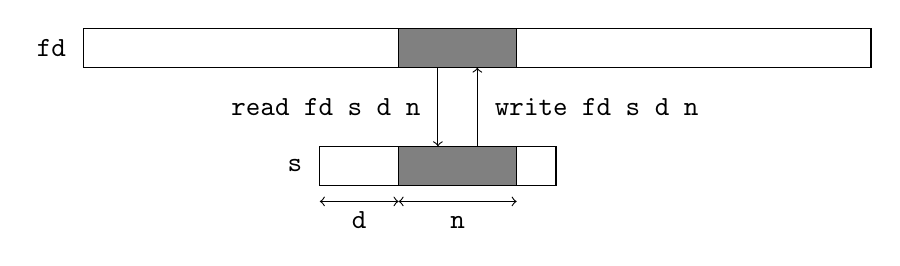
\begin{tikzpicture}[font={\ttfamily}]
\path[draw,fill=gray] (1,1.5) rectangle +(1.5, 0.5);
\path[draw] (-3,1.5) rectangle +(10, 0.5);
\node[anchor=east] at (-3.1,1.75) {fd};

\draw[->] (1.5, 1.5) to node [left=1mm] {read fd s d n} (1.5, 0.5);
\draw[<-] (2, 1.5) to node [right=1mm] {write fd s d n} (2, 0.5);

\path[draw,fill=gray] (1,0) rectangle +(1.5, 0.5);
\path[draw] (0,0) rectangle (3, 0.5);
\node[anchor=east] at (-0.1,0.25) {s};

\draw[<->] (0,-0.2) to node [below] {\phantom{n}d\phantom{n}} (1,-0.2);
\draw[<->] (1,-0.2) to node [below] {\phantom{d}n\phantom{d}} (2.5,-0.2);
\end{tikzpicture}
\end{myimage}
%
\ml+read+ and \ml+single_write+ return the number of bytes actually
read or written.

Reads and write calls are performed from the file descriptor's current
read/write position (if the file was opened in \ml+O_APPEND+ mode,
this position is set at the end of the file prior to any
writes). After the system call, the current position is advanced by
the number of bytes read or written.

For writes, the number of bytes actually written is usually the number
of bytes requested. However there are many exceptions to this
behavior: (i) if it is not possible to write the bytes (\eg if the
disk is full) (ii) the descriptor is pipe or socket in non-blocking
mode (iii) due to {\ocaml} if the write is too large. 

The reason for (iii) is that internally {\ocaml} uses auxiliary
buffers whose size is bounded by a maximal value. If this value is
exceeded the write will be partial. To work around this problem
{\ocaml} also provides the function \libvalue{Unix}{write} which
iterates the writes until all the data is written or an error occurs.
The problem is that in case of error there's no way to know the number
of bytes that were actually written. Hence \ml+single_write+ should be
preferred because it preserves the atomicity of writes (we know
exactly what was written) and it is more faithful to the original Unix
system call (note that the implementation of \ml+single_write+ is
described in section~\ref{single_write}).

%%% The french version has that here, but I don't think it belongs
%%% here.
%% In the following chapter, we shall see that when we write to a 
%% file descriptor which refers to a pipe or a lock file placed
%% in input/output blocking mode and which is then interrupted by a signal,
%% the call \ml+single_write+ returns an error \ml+EINTR+.
  
\begin{example} 
Assume \ml+fd+ is a descriptor open in write-only mode. 
%
\begin{lstlisting}
write fd "Hello world!" 3 7
\end{lstlisting}
%
writes the characters \ml+"lo worl"+ in the corresponding file,
and returns 7.
\end{example}

For reads, it is possible that the number bytes actually read is
smaller than the number of requested bytes. For example when the end
of file is near, that is when the number of bytes between the current
position and the end of file is less than the number of requested
bytes. In particular, when the current position is at the end of file,
\ml+read+ returns zero. The convention \quotes{zero equals end of
  file} also holds for special files, pipes and sockets. For example,
\ml+read+ on a terminal returns zero if we send a \ml+ctrl-D+ at the
start of a line.

Another example is when we read from a terminal. In that case,
\ml+read+ blocks until an entire line is available. If the line length
is smaller than the requested bytes \ml+read+ returns immediatly with
the line without waiting for more data to reach the number of
requested bytes. (This is the default behavior for terminals, but it
can be changed so that data is read character-by-character instead of
line-by-line, see section~\ref{sec/speciaux} and the type
\libtype{Unix}{terminal\_io} for more details.)

\begin{example} 
The following expression reads at most 100 characters from standard
input and returns them as a string.
%
\begin{lstlisting}
let buffer = String.create 100 in
let n = read stdin buffer 0 100 in
  String.sub buffer 0 n
\end{lstlisting}
\end{example}

\begin{example} 
The function \ml+really_read+ below has the same interface as
\ml+read+, but makes additional read attempts to try to get
the number of requested bytes. It raises the exception
\ml+End_of_file+ if the end of file is reached while doing this.
%
\begin{lstlisting}
let rec really_read fd buffer start length =
  if length <= 0 then () else
  match read fd buffer start length with
  | 0 -> raise End_of_file
  | r -> really_read fd buffer (start + r) (length - r);;
\end{lstlisting}
%
\end{example}

\section{Closing a descriptor}

The system call \syscall{close} closes a given descriptor.
%
\begin{listingcodefile}{tmpunix.mli}
val $\libvalue{Unix}{close}$ : file_descr -> unit
\end{listingcodefile}
% 

Once a descriptor is closed, all attempts to read, write, or do
anything else with the descriptor will fail. Descriptors should be
closed when they are no longer needed; but it is not mandatory. In
particular, and in contrasts to what happen with \ml+Pervasives+'
channels, a file descriptor doesn't need to be closed to ensure that
all pending writes have been peformed as write requests made with
\ml+write+ are immeditely transmitted to the kernel. On the other
hand, the number of descriptors allocated by a process is limited by
the kernel (from several hundreds to thousands). Doing a \ml+close+ on
an unused descriptor releases it, so that the process does not run out
of descriptors.

\section{Complete example: file copy}
\label{ex/filecopy}

We program a command \ml+file_copy+ which, given two arguments 
\ml+f1+ and \ml+f2+, copies in the file \ml+f2+ the bytes contained 
in \ml+f1+.
%
\begin{listingcodefile}{file_copy.ml}
open Unix;;

let buffer_size = 8192;;
let buffer = String.create buffer_size;;

let file_copy input_name output_name =
  let fd_in = openfile input_name [O_RDONLY] 0 in
  let fd_out = openfile output_name [O_WRONLY; O_CREAT; O_TRUNC] 0o666 in
  let rec copy_loop () =
    match read fd_in buffer 0 buffer_size with
      0 -> ()
    | r -> ignore (write fd_out buffer 0 r); copy_loop () in
  copy_loop ();
  close fd_in;
  close fd_out;;
\end{listingcodefile}
%
\begin{codefile}{copy.ml}
open Unix
open File_copy
\end{codefile}
%
\begin{listingcodefile}{copy.ml}
let copy () =
  if Array.length Sys.argv = 3 then begin
    file_copy Sys.argv.(1) Sys.argv.(2);
    exit 0
  end else begin
    prerr_endline 
      ("Usage: " ^Sys.argv.(0)^ " <input_file> <output_file>");
    exit 1
  end;;

handle_unix_error copy ();;
\end{listingcodefile}
%

The bulk of the work is performed by the the function \ml+file_copy+.
First we open a descriptor in read-only mode on the input file and
another in write-only mode on the output file. 

If the output file already exists, it is truncated (option
\ml+O_TRUNC+) and if it does not exist it is created (option
\ml+O_CREAT+) with the permissions \ml+rw-rw-rw-+ modified by creation
mask. (This is unsatisfactory: if we copy an executable file, we would
like the copy to be also executable. We will see later how to give
a copy the same permissions as the original).

In the \ml+copy_loop+ function we do the copy by blocks of
\ml+buffer_size+ bytes. We request \ml+buffer_size+ bytes to read. If
\ml+read+ returns zero, we have reached the end of file and the copy
is over. Otherwise we write the \ml+r+ bytes we have read in the
output file and start again.

Finally, we close the two descriptors. The main program \ml+copy+
verifies that the command received two arguments and passes them to
the function \ml+file_copy+.

Any error occuring during the copy results in a \ml+Unix_error+
exception which is propagated up to \ml+handle_unix_error+ which
catches and prints it. Example of errors include not being able to
open the input file because it does not exist, failure to read because
of restricted permissions, failure to write because the disk is full,
\etc

\begin{exercise} 
Add an option \ml+-a+ to the program, such that 
\ml+file_copy -a f1 f2+ appends the contents of \ml+f1+ to the end of
the file \ml+f2+. 
\end{exercise}
\begin{answer}
If the option \ml+-a+ is supplied, we need to do 
%
\begin{lstlisting}
openfile output_name [O_WRONLY; O_CREAT; O_APPEND] 0o666
\end{lstlisting}
%
instead of
%
\begin{lstlisting}
openfile output_name [O_WRONLY; O_CREAT; O_TRUNC] 0o666
\end{lstlisting}
%
Parsing the new option from the command line is left to the reader. 
\end{answer}

\section{The cost of system calls. The buffers.}

In the example \ml+file_copy+, reads were made in blocks of 8192
bytes. Why not read bytes per by bytes, or megabytes per by megabytes?
For efficiency reasons. Figure~\ref{fig/copy-speed} shows the copy
speed of \ml+file_copy+, in bytes per second, against the size of
blocks (the value \ml+buffer_size+).
\begin{myfigure}
\begin{myimage}[width="100\%"]
\begin{tikzpicture}[font=\tiny]
\pgfsetplotmarksize{0.8pt}
\draw plot[only marks,mark=*] file {data/speed-log.data};

% x-axis
\draw (0,-1) -- (7,-1);
\foreach \x in {0,...,7} { \draw (\x,-1) -- (\x,-0.95); };
\node at (0,-1.3) {\phantom{$^{2}$}1\phantom{$^{2}$}};
\node at (1,-1.3) {\phantom{$^{2}$}10\phantom{$^{2}$}};
\node at (2,-1.3) {\phantom{$^{2}$}100\phantom{$^{2}$}};
\foreach \x in {3,...,7} { \node at (\x,-1.3) {\phantom{$^{\x}$}10$^\x$}; };
\node at (8.5, -1.3) {Size (bytes)\phantom{1$^{1}$}};

% y-axis
\draw (-0.5,-0.5) -- (-0.5, 2.5);
\foreach \y in {-1,...,3} { \draw (-0.5,\y) -- (-0.45,\y); };
\node[anchor=east] at (-0.5,-1) {0.1\phantom{$^{3}$}};
\node[anchor=east] at (-0.5,0) {1\phantom{$^{3}$}};
\node[anchor=east] at (-0.5,1) {10\phantom{$^{3}$}};
\node[anchor=east] at (-0.5,2) {100\phantom{$^{3}$}};
\node[anchor=east] at (-0.5,3) {10$^{3}$};

\node[anchor=east] at (-0.5,3.5) {Speed (MB/s)};
\end{tikzpicture}
\end{myimage}
\caption{Copy speed as a function of block size}
\label{fig/copy-speed}
\end{myfigure}

For small block sizes, the copy speed is almost proportional to the
block size. But the amount of data transferred is the same regardless
of the size of the blocks. The bulk of the time is not spent in data
transfers but in the execution of the loop \ml+copy_loop+ and in the
calls to \ml+read+ and \ml+write+. By profiling more carefully we can
see that most of the time is spent in the calls to \ml+read+ and
\ml+write+. We conclude then that a system call, even if it has not
much to do (\ml+read+ read of one character), takes a minimum of about
4 micro-seconds (on the machine that was used for the test~---~a 2.8
GHz Pentium 4 ), let us say 1 to 10 microseconds.  For small
input/output blocks, the duration of the system call is what
dominates.
  
For larger blocks, between 4KB and 1MB, the copy speed is constant and
maximal. Here, the time spent in system calls and the loop is small
relative to the time spent on in the data transfer. Also the buffer
size becomes bigger than the cache sizes used by the system and the
time spent by the system to make the transfert dominates the cost of a
system call\footnote{In fact, {\ocaml} limits the size of data
  transfers to 16KB (in the current version) and repeats \ml+write+
  system calls to make the complete transfer~---~see the discussion in
  section~\ref{single_write}. But this limit is bigger than the
  size of system caches and it not observable.}

Finally, for very large blocks (8MB and more) the speed is slightly
under the maximum.  Coming into play here is the time needed to
allocate the block and assign memory pages to it as it fills up.

\begin{codefile}{speed_write.c}
#include <errno.h>
#include <string.h>
#include <caml/mlvalues.h>
#include <caml/memory.h>
#include <caml/signals.h>
#include <caml/unixsupport.h>

#define LONG_BUFFER_SIZE 9388608

CAMLprim value speed_write
        (value fd, value buf, value ofs, value len) {
  CAMLparam4(fd, buf, ofs, len);
  long numbytes;
  int ret = 0;
  char iobuf[LONG_BUFFER_SIZE];
  numbytes = Long_val(len);
  if (numbytes > LONG_BUFFER_SIZE) numbytes = LONG_BUFFER_SIZE;
  /* memmove (iobuf, &Byte(buf, Long_val(ofs)), numbytes); */
  /* enter_blocking_section (); */
  /* ret = write(Int_val(fd), iobuf, (int) numbytes); */
  ret = write(Int_val(fd), &Byte(buf, Long_val(ofs)), (int) numbytes);
  /* leave_blocking_section (); */
  if (ret == -1) uerror("write", Nothing);
  CAMLreturn (Val_int(ret));
}
\end{codefile}
%
\begin{codefile}{speed.ed}
f speed.ml
r file_copy.ml
3a
external speed_write :
   file_descr -> string -> int -> int -> int = "speed_write";;
.
/buffer_size/,/file_copy/c
let file_copy buffer_size input_name output_name =
  let buffer = String.create buffer_size in
.
/write/s/write/speed_write/
$a

let rec power n k = if k > 0 then n * power n (pred k) else 1;;
let copy () =
  if Array.length Sys.argv = 2 then begin
    let file = Sys.argv.(1) in
    let tmp = Filename.temp_file "foo" "bar" in
    let mega_octets = float (10 * (lstat file).st_size) /. 1e6 in
    (* put file in cache *)
    file_copy 10 file "/dev/null";
    for i = 23 downto 0 do 
      let start = let t = Unix.times () in t.tms_utime +. t.tms_stime in
      let block = power 2 i in
      for i = 1 to 10 do file_copy block file tmp done;
      let stop = let t = Unix.times () in t.tms_utime +. t.tms_stime in
      let time = stop -. start in
      let speed = mega_octets /. time in
      Printf.printf "%9d %.2f" block speed; 
      print_newline ();
    done;
      exit 0
  end else begin
    prerr_endline ("Usage: " ^Sys.argv.(0)^ " <input_file> <output_file>");
    exit 1
  end;;

handle_unix_error copy ();;
.
wq
\end{codefile}
% $

Moral of the story, a system call, even if it does very little work,
costs dearly~---~much more than a normal function call: roughly, 2 to
20 microseconds for each system call, depending on the the
architecture. It is therefore important to minimize de number of
system calls. In particular, read and write operations should be made
in blocks of reasonable size and not character by character.

In examples like \ml+file_copy+, it is not difficult to do input/ouput
with large blocks. But other types of programs are more naturally
written with character by character input (\eg{} reading a line from a
file, lexical analysis \etc), and displaying some characters at once
(\eg{} display a number).  To satisfy the needs of these programs,
most systems provide input/output libraries with an additional layer
of software between the application and the operating system. For
example, in {\ocaml} the \ml+Pervasives+ module defines the abstract
types \libtype{Pervasives}{in\_channel} and
\libtype{Pervasives}{out\_channel}, similar to file descriptors, and
functions on these types like \libvalue{Pervasives}{input\_char},
\libvalue{Pervasives}{input\_line},
\libvalue{Pervasives}{output\_char}, or
\libvalue{Pervasives}{output\_string}.  This layer uses buffers to
group sequences of character by character reads or writes into a
single read or write. This results in better performance for programs
that proceed character by character.  Moreover this additional layer
makes programs more portable: we just need to implement this layer
with the system calls provided by another operating system to port all
the programs that use this library on this new platform.

\section{Complete example: a small input/output library}

Here is an implementation of a part of the {\ocaml} \ml+Pervasives+ library to illustrate read/write
techniques by buffer. The interface is the following:
%
\begin{listingcodefile}{io.mli}
exception End_of_file

type in_channel
val open_in : string -> in_channel
val input_char : in_channel -> char
val close_in : in_channel -> unit

type out_channel
val open_out : string -> out_channel
val output_char : out_channel -> char -> unit
val close_out : out_channel -> unit
\end{listingcodefile}
%
We start with the \quotes{read} part. The abstract type 
\ml+in_channel+ is implemented as follows: 
%
\begin{listingcodefile}{io.ml}
open Unix;;

type in_channel =
  { in_buffer: string;
    in_fd: file_descr;
    mutable in_pos: int;
    mutable in_end: int };;
exception End_of_file
\end{listingcodefile}
%

The character string in the field \ml+in_buffer+ is literally the buffer.
The field \ml+in_fd+ is a file descriptor 
(Unix), opened on the file during the read. The field 
\ml+in_pos+ is the current position of the read cursor in the buffer .  The
field \ml+in_end+ is the number of valid characters in the buffer.
%
\begin{myimage}[width="85\%"]
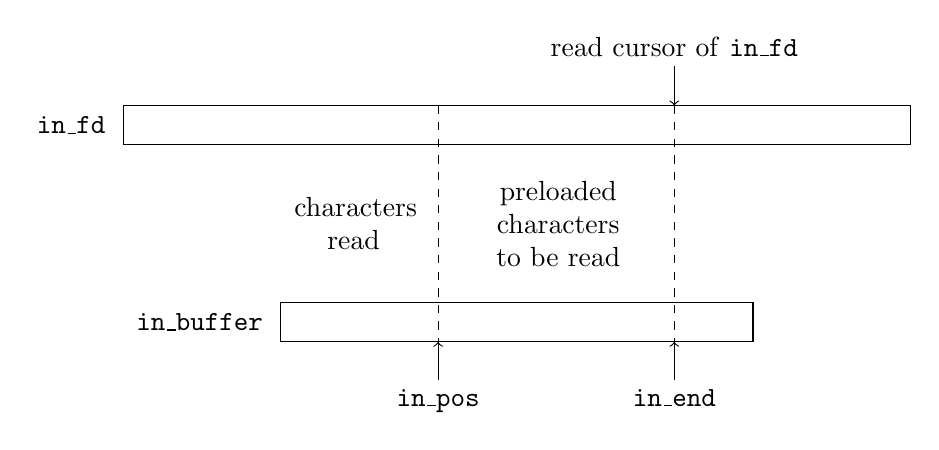
\begin{tikzpicture}
\path[draw] (-3,2.5) rectangle +(10, 0.5);
\node[anchor=east] at (-3.1,2.75) {\texttt{in\_fd}};
\draw[dashed] (1,3) to node [left=2mm,text width=1.5cm,text centered] 
 {characters read} (1,0);

\draw[dashed] (4,3) to node [left=1mm,text width=2.5cm,text centered] 
 {preloaded characters to be read} (4,0);

\path[draw] (-1,0) rectangle +(6, 0.5);
\node[anchor=east] at (-1.1,0.25) {\texttt{in\_buffer}};

\node (fdpos) at (4,3.75) {read cursor of \texttt{in\_fd}};
\draw[->] (fdpos.south) to (4,3);

\node (ipos) at (1,-0.75) {\texttt{\phantom{d}in\_pos\phantom{d}}};
\node (iend) at (4,-0.75) {\texttt{\phantom{p}in\_end\phantom{p}}};
\draw[->] (ipos.north) to (1,0);
\draw[->] (iend.north) to (4,0);
\end{tikzpicture}
\end{myimage}

The field \ml+in_pos+ and \ml+in_end+ will be modified in place during 
read operations ; we therefore declare then as \ml+mutable+.
%
\begin{listingcodefile}{io.ml}
let buffer_size = 8192;;
let open_in filename =
  { in_buffer = String.create buffer_size;
    in_fd = openfile filename [O_RDONLY] 0;
    in_pos = 0;
    in_end = 0 };;
\end{listingcodefile}
%
At the opening of a file in read mode, we create a buffer of
reasonable size (large enough so as not to make too many
system calls; small enough so as not to waste memory). We
then initialize the field \ml+in_fd+ with a Unix file descriptor
opened in read mode on the file in question. The 
buffer is initially empty (It does not contain any characters from the file); 
the field \ml+in_end+ is therefore initialized to zero.
%
\begin{listingcodefile}{io.ml}
let input_char chan =
  if chan.in_pos < chan.in_end then begin
    let c =  chan.in_buffer.[chan.in_pos] in
      chan.in_pos <- chan.in_pos + 1;
      c
  end else begin
    match read chan.in_fd chan.in_buffer 0 buffer_size
    with 0 -> raise End_of_file
       | r -> chan.in_end <- r;
              chan.in_pos <- 1;
              chan.in_buffer.[0]
  end;;
\end{listingcodefile}
%

To read a character from \ml+in_channel+, we do one of two things. 
Where there is at least one character in the buffer;
that is to say, the field \ml+in_pos+ is less than the field 
\ml+in_end+. Then we return the next character in the buffer, that which
is in position  \ml+in_pos+, and we increment \ml+in_pos+. Where the buffer
is empty. We make a system call \ml+read+ to refill the 
buffer. If \ml+read+ returns zero, that means we have reached 
the end of the file so we then raise an \ml+End_of_file+ exception. Otherwise,
we put the number of characters read in the field \ml+in_end+. (We could 
have received less characters than we requested, and thus the buffer 
could have been partially refilled.) Then we return the first of the  
characters read.
%
\begin{listingcodefile}{io.ml}
let close_in chan =
  close chan.in_fd;;
\end{listingcodefile}
%
The closing of an \ml+in_channel+ is reduced to the closing of the underlying Unix descriptor. 

The \quotes{writing} part is very similar to the \quotes{reading} part. The 
only asymmetry is that the buffer now contains incomplete writes 
(characters that have already been buffered but not written to the file descriptor),
and not reads in advance (characters that have buffered, but not yet read).

\begin{myimage}[width="85\%"]
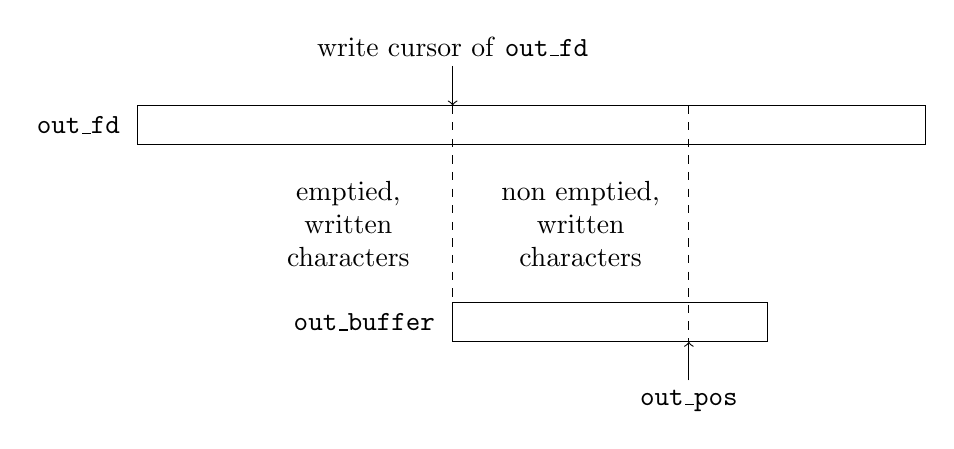
\begin{tikzpicture}
\path[draw] (-3,2.5) rectangle +(10, 0.5);
\node[anchor=east] at (-3.1,2.75) {\texttt{out\_fd}};
\draw[dashed] (1,3) to node [left=2mm,text width=2cm,text centered] 
 {emptied, written characters} (1,0);

\draw[dashed] (4,3) to node [left,text width=2.5cm,text centered] 
 {non emptied, written characters} (4,0);

\path[draw] (1,0) rectangle +(4, 0.5);
\node[anchor=east] at (0.9,0.25) {\texttt{out\_buffer}};

\node (fdpos) at (1,3.75) {write cursor of \texttt{out\_fd}};
\draw[->] (fdpos.south) to (1,3);

\node (opos) at (4,-0.75) {\texttt{out\_pos}};
\draw[->] (opos.north) to (4,0);
\end{tikzpicture}
\end{myimage}
%
\begin{listingcodefile}{io.ml}
type out_channel =
  { out_buffer: string;
    out_fd: file_descr;
    mutable out_pos: int };;

let open_out filename =
  { out_buffer = String.create 8192;
    out_fd = openfile filename [O_WRONLY; O_TRUNC; O_CREAT] 0o666;
    out_pos = 0 };;

let output_char chan c =
  if chan.out_pos < String.length chan.out_buffer then begin
    chan.out_buffer.[chan.out_pos] <- c;
    chan.out_pos <- chan.out_pos + 1
  end else begin
    ignore (write chan.out_fd chan.out_buffer 0 chan.out_pos);
    chan.out_buffer.[0] <- c;
    chan.out_pos <- 1
  end;;

let close_out chan =
  ignore (write chan.out_fd chan.out_buffer 0 chan.out_pos);
  close chan.out_fd;;
\end{listingcodefile}
%
 
To write a character to an \ml+out_channel+, where the buffer 
is not full, it suffices to store the character in the buffer
in the position \ml+out_pos+, and to advance \ml+out_pos+; when 
the buffer is full, we empty the buffer with 
a call to \ml+write+, then we store the character to write at the beginning of 
the buffer.

When we close an \ml+out_channel+, we should not forget to dump  
the buffer contents (the characters between the positions 0 included and 
\ml+out_pos+ excluded) into the file. Otherwise, the writes 
made after the last dump will be lost.

\begin{exercise} 
Implement a function 
%
\begin{lstlisting}
val output_string : out_channel -> string -> unit
\end{lstlisting}
%
which behaves like a series of \ml+output_char+ on each 
character of the string, but is more efficient.
\end{exercise}
\begin{answer}
The idea is to copy the string to be output into the buffer. We need to 
take into account the case where there is not enough space in the buffer
(in that case the buffer needs to emptied), and also the case where the string is  
longer than the buffer can hold (in that case it is necessary to write it directly). 
Here is a possible solution. 
%
\begin{codefile}{ex2.ml}
open Unix;;
\end{codefile}
%
\begin{listingcodefile}{ex2.ml}
let output_string chan s =
  let avail = String.length chan.out_buffer - chan.out_pos in
  if String.length s <= avail then begin
    String.blit s 0 chan.out_buffer chan.out_pos (String.length s);
    chan.out_pos <- chan.out_pos + String.length s
  end
  else if chan.out_pos = 0 then begin
    ignore (write chan.out_fd s 0 (String.length s))
  end
  else begin
    String.blit s 0 chan.out_buffer chan.out_pos avail;
    let out_buffer_size = String.length chan.out_buffer in
    ignore (write chan.out_fd chan.out_buffer 0 out_buffer_size);
    let remaining = String.length s - avail in
    if remaining < out_buffer_size then begin
      String.blit s avail chan.out_buffer 0 remaining;
      chan.out_pos <- remaining
    end else begin
      ignore (write chan.out_fd s avail remaining);
      chan.out_pos <- 0
    end
  end;;
\end{listingcodefile}
%
\begin{codefile}{ex2.ml}
let ex2 () = 
  if Array.length Sys.argv < 3 then begin 
     prerr_string "Usage: test <sources> <dest>"; 
     exit 2;
  end;
  let fdin = open_in Sys.argv.(1) in
  let fdout = open_out Sys.argv.(2) in
  prerr_endline "copying";
  try while true do output_char fdout (input_char fdin) done
  with End_of_file -> 
   prerr_endline "Done";
   output_string fdout "The end.\n";
   prerr_endline "Closing";
   close_out fdout;;

handle_unix_error ex2 ();;
\end{codefile}
%
\begin{codefile}{ex2.test}
./ex2.byte ex2.ml ex2.out
(cat ex2.ml; echo "C'est la fin.") | diff --brief - ex2.out
rm ex2.out
\end{codefile}
\end{answer}


\section{Positioning}

The system call \syscall{lseek} permits changing the current position of the read/write cursor.
%
\begin{codefile}{tmpunix.mli}
type seek_command = Unix.seek_command
\end{codefile}
%
\begin{listingcodefile}{tmpunix.mli}
val $\libvalue{Unix}{lseek}$ : file_descr -> int -> seek_command -> int
\end{listingcodefile}
%

The first argument is the first descriptor and the second argument is
the position offset specifier. This is interpreted differently
depending on the value of the third argument, which indicates the type
of position desired:
%
\begin{mltypecases}
\begin{tabular}{@{}lp{0.8\textwidth}}
\ml+SEEK_SET+ & Absolute position. The second argument is the
index into the file, in characters, to position the pointer at. The
first character of a file is at position zero. \\
%
\ml+SEEK_CUR+ & Position relative to the current position. 
The second argument is a displacement relative to the  
current position. This may be negative to move backwards or positive
to move forwards. \\
%
\ml+SEEK_END+ & Position relative to the end of file. The 
second argument is a displacement relative to the end of file.
As for \ml+SEEK_CUR+, this may be negative as well as
positive.
\end{tabular}
\end{mltypecases}
%
The value returned by \ml+lseek+ is the absolute position of the
read/write cursor (after it has actually been positioned).

An error is triggered if the absolute position requested is negative.
On the other hand, the position requested could well be located after
the end of file. Right after such a positioning, a  \ml+read+
returns zero (end of file reached); an \ml+write+ extends the file 
from the zero up to the position requested, then writes the supplied data. 

\begin{example} 
To position the cursor on the 1000th character of a file:
%
\begin{lstlisting}
lseek fd 1000 SEEK_SET
\end{lstlisting}
%
To rewind by one character:
%
\begin{lstlisting}
lseek fd (-1) SEEK_CUR
\end{lstlisting}
%
To find the size of a file:
%
\begin{lstlisting}
let file_size = lseek fd 0 SEEK_END in ...
\end{lstlisting}
\end{example}

For descriptors opened in \ml+O_APPEND+ mode, the read/write cursor is 
automatically placed at the end of the file before each write. 
Thus the call \ml+lseek+ is useless for writing 
on such a descriptor. On the other hand, it is well taken into account
by the read. 

The behavior of \ml+lseek+ is unpredictable on certain type of files
for which direct access is meaningless: communication devices (pipes, lock files),
but also most special files (peripherals), such as for example the terminal.
For most implementations of Unix, an \ml+lseek+ on such files 
is simply ignored:  The read/write cursor is positioned 
but read/write operations ignore it.
In some implementations, \ml+lseek+ on a pipe or on a lock file
triggers an error.

\begin{exercise}
The command \ml+tail+ displays the $n$ last lines of a file.
How should it be efficiently implemented if the file in question is
a normal file? How should it be done to cope with other types of files?
How to add the option \ml+-f+ (cf. \ml+man tail+)?
\end{exercise}
\begin{answer}
The naive implementation of \ml+tail+ is to read the file
sequentially from the beginning keeping the last $n$ lines read in
a circular buffer. When we reach the end of file, we display the buffer. 
When the data comes from a pipe or a special file which
does not implement \ml+lseek+, there is no better way.
On the other hand, if the data is coming from a normal file,
it would be better to read the file starting from the end: with 
\ml+lseek+, we read the last 4096 characters:  We scan them for 
the end of line;hr.  If there are at least $n$, we output and display
the corresponding lines.  Otherwise, we start again with the preceding
4096 characters, \etc

To add the option \ml+-f+,it suffices to at once display the last 
$n$ lines, to position the cursor at the end of the file and to
attempt to read (through \ml+read+) starting from it. If \ml+read+
succeeds to read something, we display it immediately and begin again.
If \ml+read+ returns 0, we wait a little (\ml+sleep 1+) then 
try again. 
\end{answer}

\section{Operations specific to certain file types}

In Unix, data communication is done via file descriptors representing
either permanent files (files, peripherals) or volatile ones (pipes
and sockets, see chapters~\ref{sec/pipes} and \ref{sec/sockets}). File
descriptors provide a uniform and media-independent interface for data
communication. Of course the actual implementation of the operations
on a file descriptor depends on the underlying media.

However this uniformity breaks when one needs to access all the
features provided by a given media. General operations (opening,
writing, reading, \etc) remain uniform on most descriptors but even,
on certain special files, these may have an ad hoc behavior defined
by the kind of peripheral and its parameters. There are also
operations that work only with certain kind of media.

\subsection*{Normal files}

We can shorten an ordinary file through the system calls
\syscall{truncate} and \syscall{ftruncate}.
%
\begin{listingcodefile}{tmpunix.mli}
val $\libvalue{Unix}{truncate}$  : string -> int -> unit
val $\libvalue{Unix}{ftruncate}$ : file_descr -> int -> unit
\end{listingcodefile}
%

The first argument is the file to truncate (specified either by its
name or by a file descriptor open on the file). The second argument is the
desired size. All the data after this position is lost.

\subsection*{Symbolic links}

Most of the the operations on files \quotes{follow} symbolic 
links: that is to say, they are applied to files to which 
the symbolic link points, and not on the symbolic link 
itself. Examples: \indexvalue{openfile}, \indexvalue{stat},
\indexvalue{truncate}, \indexvalue{opendir}. We have two 
operations, \syscall{symlink} and \syscall{readlink} on symbolic
links:
%
\begin{listingcodefile}{tmpunix.mli}
val $\libvalue{Unix}{symlink}$  : string -> string -> unit
val $\libvalue{Unix}{readlink}$ : string -> string
\end{listingcodefile}
%
The call \ml+symlink f1 f2+ creates the file \ml+f1+ as the symbolic 
link of \ml+f2+ (like the command \ml+ln -s f1 f2+). The call 
\ml+readlink+ returns the content of a symbolic link, that is to say a 
the name of the file to which it points.

\subsection*{Special files\label{sec/speciaux}}

Special files may be of type \quotes{character} or of type
\quotes{block}.  The first are for reading and writing characters: we
cannot read or write characters expect in sequence. These character
devices are typically terminals, the peripherals are, printers, \etc{}
The block devices, typically disks, are a permanent or temporary
resource; characters are read in blocks given in absolute form or
relative with respect to the current position. Among the special files,
we may distinguish:
\begin{mltypecases}
\begin{tabular}{@{}lp{0.8\textwidth}}
\ml+/dev/null+ & This is the black hole which swallows
  everything we put into and from which nothing comes out. Extremely
  useful for ignoring the results of a process: we redirect its output
  to \ml+/dev/null+ (see the chapter~\ref{sec/pipes}).\\
%
\ml+/dev/tty*+ & These are the terminals. \\
%
\ml+/dev/pty*+ & These are the pseudo-terminals: They are not real
  terminals but provide the same interface. \\
%
\ml+/dev/hd*+ & These are the disks. \\
%
\ml+/proc+ & Under Linux, system parameters organized as a
  file system. Allows to read and write them.
\end{tabular}
\end{mltypecases}

The usual file system calls on special files can behave differently.
However, most special files (terminals, tape drives, disks, \ldots)
follow \ml+read+ and \ml+write+ in the obvious manner (but sometimes
with restrictions on the number of bytes written or read), but many
ignore \indexvalue{lseek}.

In addition to the usual file system calls, special files which
represent peripherals must be commanded and/or configured
dynamically. For example, for a tape drive, rewind or fast forward the
tape; for a terminal terminal, choice of the line editing mode,
behaviour of special characters, serial connection parameters (speed,
parity, \etc).  These operations are made in Unix through the system
call \syscall{ioctl} which group together all the particular
cases. However, this system call is not provided by {\ocaml}; it is
ill-defined and cannot be treated in a uniform way.

\subsubsection{Terminals}
\label{sec/termio}


Terminals and  pseudo-terminals are character accessible special files
for which 
{\ocaml} allows configuration access. The call \syscall{tcgetattr}
takes as an argument an open file descriptor on the special file 
in question and returns a structure of type
\ml+terminal_io+ which describe the state of the terminal
represented by the file according to the standard  \textsc{posix}.
%
\begin{codefile}{tmpunix.mli}
type terminal_io = Unix.terminal_io
\end{codefile}
%
\begin{lstlisting}
type $\libtype{Unix}{terminal\_io}$ = 
  { c_ignbrk : bool; c_brk_int : bool; ...;  c_vstop : char }
\end{lstlisting}
%
\begin{listingcodefile}{tmpunix.mli}
val $\libvalue{Unix}{tcgetattr}$ : file_descr -> terminal_io
\end{listingcodefile}
%
This structure may be modified then passed to the function 
\syscall{tcsetattr} to change the attributes of the peripheral.
%
\begin{codefile}{tmpunix.mli}
type setattr_when = Unix.setattr_when
\end{codefile}
%
\begin{listingcodefile}{tmpunix.mli}
val $\libvalue{Unix}{tcsetattr}$ : file_descr -> setattr_when -> terminal_io -> unit
\end{listingcodefile}
%
The first argument is the file descriptor of the peripheral. 
The last argument is a structure of type 
\ml+tcgetattr+ describing the parameters of the peripheral such that are  
needed for setup.  The second argument is a flag of type enumeration.
\ml+setattr_when+ indicating the moment from which the change 
should take effect: immediately (\ml+TCSANOW+), after having transmitted
all written data (\ml+TCSADRAIN+) or after having read all the data 
received (\ml+TCAFLUSH+).  The choice \ml+TCSADRAIN+ is
recommended for changing the write parameters and \ml+TCSAFLUSH+
for modifying the read parameters. 

\begin{example}
During the reading of a password, characters entered by the user should not
be echoed to the terminal or pseudo-terminal.
%
\begin{codefile}{passwd.ml}
open Unix;;
\end{codefile}
%
\begin{listingcodefile}{passwd.ml}
let read_passwd message = 
  match
    try 
      let default = tcgetattr stdin in
      let silent = 
        { default with 
          c_echo = false; 
          c_echoe = false; 
          c_echok = false; 
          c_echonl = false; 
        } in
      Some (default, silent) 
    with _ -> None
  with 
  | None -> input_line Pervasives.stdin
  | Some (default, silent) -> 
      print_string message; 
      flush Pervasives.stdout;
      tcsetattr stdin TCSANOW silent;
      try 
        let s = input_line Pervasives.stdin in 
        tcsetattr stdin TCSANOW default; s
      with x -> 
        tcsetattr stdin TCSANOW default; raise x;;
\end{listingcodefile}
%

The \ml+read_passwd+ function begins by recovering the default value  
of the terminal associated with \ml+stdin+ and constructing 
a modified version in which the characters entered are not echoed.  
In case of failure, when the input stream is not a terminal,
it is enough to read a line. Otherwise we display
a message, we change the terminal, we read the response and reset the  
terminal into its normal state. Care has to be taken to set
the terminal back to its normal state after a read failure.
\end{example}
%
Sometimes a program needs to launch another linked to its
input stream from a terminal (or pseudo-terminal).  {\ocaml} does not
have any support for this \footnote {The Cash library
~\cite {Cash} supplies such functions.} so it is necessary to manually
look for an unused pseudo-terminals  (in general, they are files 
with names in the form of \ml+/dev/tty[a-z][a-f0-9]+) and find one of 
these files which has not already been opened, open it and launch  
the application with this file in the input stream.

Four other functions allow control of the stream (flush data on hold,
wait for end of transmission, restart communication). 
%
\begin{listingcodefile}{tmpunix.mli}
val $\libvalue{Unix}{tcsendbreak}$ : file_descr -> int -> unit
\end{listingcodefile}
%
The function  \syscall{tcsendbreak} sends an interrupt to the 
peripheral. Its second argument is the length of the interrupt
(\ml+0+ is interpreted as the default value for the 
peripheral).
%
\begin{listingcodefile}{tmpunix.mli}
val $\libvalue{Unix}{tcdrain}$ : file_descr -> unit
\end{listingcodefile}
%
The function \syscall{tcdrain} waits for all the data written to be 
transmitted.
%
\begin{codefile}{tmpunix.mli}
type flush_queue = Unix.flush_queue
\end{codefile}
%
\begin{listingcodefile}{tmpunix.mli}
val $\libvalue{Unix}{tcflush}$ : file_descr -> flush_queue -> unit
\end{listingcodefile}
%
Depending on the flag passed as the second argument, a call to the
function \syscall{tcflush} abandons the data written but not yet
transmitted
(\ml+TCIFLUSH+), or the data received but not yet read 
(\ml+TCOFLUSH+) or both (\ml+TCIOFLUSH+).
%
\begin{codefile}{tmpunix.mli}
type flow_action = Unix.flow_action
\end{codefile}
%
\begin{listingcodefile}{tmpunix.mli}
val $\libvalue{Unix}{tcflow}$ : file_descr -> flow_action -> unit
\end{listingcodefile}
%

Depending on the flag passed as the second argument, a call to the
function \syscall{tcflow} suspends the emission (\ml+TCOOFF+), restarts 
the emission (\ml+TCOON+), sends a control character \textsc{stop}
or \textsc{start} to request that the transmission be suspended
(\ml+TCIOFF+) or restarted (\ml+TCION+).
%
\begin{listingcodefile}{tmpunix.mli}
val $\libvalue{Unix}{setsid}$ : unit -> int
\end{listingcodefile}
%
The function \syscall{setsid} puts the process in a new
session and detaches it from the terminal.

\section{Locks on files}

If two processes attempt to modify the same file in parallel there is a
danger that some of the writes may collide with each other. In some cases, opening
the file in \ml+O_APPEND+ mode allows these collisions to be managed, for example,
in the case of a \ml+log+ file where data is always written 
at the end of the file.   However, this mechanism
does not resolve the general case where the writes are at  
arbitrary positions in the file, for example, when a file represents a
database. It then becomes necessary for all the processes utilizing this file
to collaborate so as not to step on each others toes.
A lock on the file is always possible by creating an auxiliary lock file
(see page \pageref{page/lock}). The system call 
\syscall{lockf} allows a part of the file to be locked thereby providing
very accurate synchronization.
%
\begin{codefile}{tmpunix.mli}
type lock_command = Unix.lock_command
\end{codefile}
%
\begin{listingcodefile}{tmpunix.mli}
 val $\libvalue{Unix}{lockf}$ : file_descr -> lock_command -> int -> unit
\end{listingcodefile}


\section{Complete example: recursive copy of files}
\label{sec/copyrec}

We will extend the function \ml+file_copy+ (section~\ref{ex/filecopy})
to copy symbolic links and directories in addition to normal files. 
In the case of directories, we need copy their contents recursively.

We begin by reusing the function \ml+file_copy+ in the example of the same name
for copying normal files (page~\pageref{ex/filecopy}). 
\begin{lstlisting}
open Unix
...
let file_copy input_name output_name =
...
\end{lstlisting}
The function \ml+set_infos+ below modifies the owner, the  
access rights and  the last dates of access/last modification
of a file. Its purpose is to preserve this information during the copy.

%
\begin{codefile}{copy_rec.ml}
open Unix;;
open File_copy;;
\end{codefile}
%
\begin{listingcodefile}{copy_rec.ml}
let set_infos filename infos =
  utimes filename infos.st_atime infos.st_mtime;
  chmod filename infos.st_perm;
  try
    chown filename infos.st_uid infos.st_gid
  with Unix_error(EPERM,_,_) -> ()
\end{listingcodefile}
%
The system call \ml+utime+ modifies the dates of access and 
modification.  We use \ml+chmod+ and \ml+chown+ to re-establish 
the access rights and the owner. For normal users, there are  
a certain number of cases where  \ml+chown+ will fail with an error
\quotes{permission denied}.  We trap this error and ignore it.

Here's the main recursive function. 
\begin{listingcodefile}{copy_rec.ml}
let rec copy_rec source dest =
  let infos = lstat source in
  match infos.st_kind with
    S_REG ->
      file_copy source dest;
      set_infos dest infos
  | S_LNK ->
      let link = readlink source in
      symlink link dest
  | S_DIR ->
      mkdir dest 0o200;
      Misc.iter_dir
        (fun file ->
          if file <> Filename.current_dir_name 
              && file <> Filename.parent_dir_name 
          then 
            copy_rec
              (Filename.concat source file)
              (Filename.concat dest file))
        source;
      set_infos dest infos
  | _ ->
      prerr_endline ("Can't cope with special file " ^ source)
\end{listingcodefile}

We begin by reading the information from the source file. If this is a 
normal file, we copy its contents with \ml+file_copy+, then its 
information with \ml+set_infos+. If it is a symbolic link, we read
where it points to, and we then create a link which points to the same 
object.  If it is a directory, we create a directory as the
destination, then we read the directory entries in the source (ignoring
the entries which are about the source  \ml+Filename.current_dir_name+
or its parent directory \ml+Filename.parent_dir_name+, which we should 
certainly not copy), then we recursively call \ml+copy+ for 
each entry.  We ignore the other type of files, and include a  
warning.

The main program is relatively straight forward:
%
\begin{codefile}{copyrec.ml}
open Unix
open Copy_rec
\end{codefile}
%
\begin{listingcodefile}{copyrec.ml}
let copyrec () =
  if Array.length Sys.argv <> 3 then begin
    prerr_endline ("Usage: " ^Sys.argv.(0)^ " <source> <destination>");
    exit 2
  end else begin
    copy_rec Sys.argv.(1) Sys.argv.(2);
    exit 0
  end
;;
handle_unix_error copyrec ();;
\end{listingcodefile}

\begin{exercise} 
\label{ex/copyrec}
Intelligently copy hard links. As is described in the following,
\ml+copyrec+ creates $n$ duplicates of the same file which appears under $n$
different names in the hierarchy of files to copy. Try to detect this
situation and try not to copy the file more than once. 
Make hard links in the target hierarchy.
\end{exercise}

\begin{answer}
It is necessary to keep a table of source files that have already been copied, for which  
the tuple \ml+(st_dev, st_ino)+ for each source file corresponds with  
the name of its destination file. For each copy, we look up this
table to see if a source file with the same tuple
\ml+(st_dev,st_ino)+ had already been copied; if yes, we make a hard link  
to the target file, instead of repeating the copy. To minimize 
the size of this table, we can insert only the files 
which have more than one name, that is to say those where \ml+st_nlink > 1+.
%
\begin{codefile}{copyrec_ex.ml}
open File_copy
open Copy_rec
open Sys
open Unix
\end{codefile}
%
\begin{listingcodefile}{copyrec_ex.ml}
let copied_files = (Hashtbl.create 53 : ((int * int), string) Hashtbl.t)

let rec copy source dest =
  let infos = lstat source in
  match infos.st_kind with
    S_REG ->
      if infos.st_nlink > 1 then begin
        try
          let dest' = 
            Hashtbl.find copied_files (infos.st_dev, infos.st_ino)
          in link dest' dest
        with Not_found ->
          Hashtbl.add copied_files (infos.st_dev, infos.st_ino) dest;
          file_copy source dest;
          set_infos dest infos
      end else begin
        file_copy source dest;
        set_infos dest infos
      end
\end{listingcodefile}
\begin{lstlisting}
  | S_LNK -> ...
\end{lstlisting}
\begin{codefile}{copyrec_ex.ml}
| _ -> ()
\end{codefile}
\end{answer}

\section{Example: {\normalfont\texttt{T}}ape {\normalfont\texttt{AR}}chive}

The \ml+tar+ format (for \ml+t+ape \ml+ar+chive) allows us to represent 
a group of files in one file.  (In addition it allows us to store 
an entire file hierarchy on a tape.)  The tar archive may be viewed as
a mini file system. 

In this section we describe a group of functions which 
allows the reading and writing of archives in the \ml+tar+ format. The  
first part for which a complete example is provided, consists of writing a function
\ml+readtar+ such that  \ml+readtar a+ displays the list of files 
contained in the archive~\ml+a+  and \ml+readtar a f+ displays the contents of  
the file \ml+f+ contained within the archive \ml+a+. We leave as an 
exercise the problem of extracting all the files contained in an archive
as well as generating an archive starting from a group of files.

\paragraph{Description of format}

A \ml+tar+ archive is a set of records, with each 
record representing a file.  A record is composed of a header
which encodes the information about the file (its name, type, size, owner \etc) 
and the contents of the file.
The header consists of a block (512 bytes) as shown in the table~\ref {fig/tar}.
\begin{mytable}
\begin{tabular}{rrlll}
Offset & Length & Code Type & Name & Description \\
\hline
  0&   100 & string  &  \ml+name+   & file name \\
100&     8 & octal   &  \ml+perm+   & file access modes\\
108&     8 & octal   &  \ml+uid+    & id of user\\
116&     8 & octal   &  \ml+gid+    & id of group of the user\\
124&    12 & octal   &  \ml+size+   & file size (in bytes)\\
136&    12 & octal   &  \ml+mtime+  & Date of last modification\\
148&     8 & octal   &  \ml+checksum+ & Header checksum \\
156&     1 &character&  \ml+kind+   & File type  \\
157&   100 & octal   &\emph{\ml+link+}   & Link\\
257&     8 & string  &  \ml+magic+  & Signature (\ml+"ustar\032\032\0"+)\\
265&    32 & string  &  \ml+user+   & Name of user\\
297&    32 & string  &  \ml+group+  & Name of user's group\\
329&     8 & octal   &\emph{\ml+major+}  & Peripheral major number\\
337&     8 & octal   &\emph{\ml+minor+}  & Peripheral minor number\\
345&   167 &         &         & Padding \smallskip\\
\hline 
\end{tabular}
\begin{flushleft}
\small\textbf{Note.}\quad Field lengths are in number of
bytes. All fields are encoded with character strings terminated with
the null character \ml+'\000'+; excepting the field \ml+kind+ and
\ml+size+ (\ml+'\000'+ optional).
\end{flushleft}
\ifnothtml{\vspace{-\onelineskip}}
\caption {Header structure}
\label{fig/tar}
\end{mytable}

The contents are represented by a number of whole blocks following the header. 
The records are given one after another. If necessary, the file is padded
with empty blocks in order to reach a minimum of 20 blocks. 

As tar archives are designed to be written to unreliable media and
retrieved many years later, the header contains a \ml+checksum+ field
which allows the archives to be found when the header is damaged (or
to use more than one file as an archive.) The checksum value is the
sum of the character codes in the header (from this, we hypothesize
that the \ml+checksum+ field which is not yet calculated consists of
blanks terminated by the null character).

The \ml+kind+ field encodes the file type in a byte.
Significant values are the characters indicated in the table 
below\footnote {This field can also take different values to encode
  pathological cases, for example, when the value of a field exceeds
  the place reserved for it in the header or in the extensions of the
  \ml+tar+ command.}:
%
\begin{center}
\begin{tabular}{cccccccc}
\ml+'\0'+ or \ml+'0'+ & 
\ml+'1'+ & \ml+'2'+ &\ml+'3'+ & \ml+'4'+ & \ml+'5'+ & \ml+'6'+ & \ml+'7'+\\
\hline
\ml+REG+ & 
\ml+LINK+ & 
\ml+LNK+ & 
\ml+CHR+ & 
\ml+BLK+ & 
\ml+DIR+ & 
\ml+FIFO+ &
\ml+CONT+
\end{tabular}
\end{center}
Most of the cases correspond to the Unix file type \ml+st_link+.
\ml+LINK+ represents hard links; these have 
the same node (\emph{inode}) but are accessible through two different paths.
In this case,the link must lead to another
file already defined within the archive. \ml+CONT+ represents an 
ordinary file, but which is represented by a contiguous memory zone
(this is a feature of some types of file systems, we can then treat it
like an ordinary file).

The field 
\emph{\ml+link+} represents the link when the value of \ml+kind+ equals \ml+LNK+ or 
\ml+LINK+.  The fields \emph{\ml+major+} and \emph{\ml+minor+}
contain the major and minor numbers of the peripheral in the case 
where the value of the field \ml+kind+ equals \ml+CHR+ or \ml+BLK+. These three fields are
not used in other cases.

The value of the field \ml+kind+ is naturally represented by a variant type;
the header by a record:
%
\begin{codefile}{tarlib.ml}
open Unix;;
\end{codefile}
%
\begin{listingcodefile}{tarlib.ml}
type kind =
  | REG | LNK of string | LINK of string | CHR of int * int 
  | BLK of int * int | DIR | FIFO | CONT

type header = 
    { name : string; perm : int; uid : int; gid : int; size : int; 
      mtime : int; kind : kind; user : string; group : string } 
\end{listingcodefile}

\paragraph {Reading a header}
Reading a header is not very interesting, but 
cannot be ignored.
%
\begin{listingcodefile}{tarlib.ml}
exception Error of string * string
let error err mes = raise (Error (err, mes));;
let handle_error f s = 
  try f s with 
  | Error (err, mes) -> 
      Printf.eprintf "Error: %s: %s" err mes;
      exit 2
        
let substring s offset len = 
  let max_length = min (offset + len + 1) (String.length s) in
  let rec real_length j =
    if j < max_length && s.[j] <> '\000' then real_length (succ j) 
    else j - offset in
  String.sub s offset (real_length offset);;

let integer_of_octal nbytes s offset =
  let i = int_of_string ("0o" ^ substring s offset nbytes) in
  if i < 0 then error "Corrupted archive" "integer too large" else i;;

let kind s i =
  match s.[i] with
  | '\000' | '0' -> REG
  | '1' -> LINK (substring s (succ i) 99)
  | '2' -> LNK (substring s (succ i) 99)
  | '3' -> CHR (integer_of_octal 8 s 329, integer_of_octal 8 s 329)
  | '4' -> BLK (integer_of_octal 8 s 329, integer_of_octal 8 s 337)
  | '5' -> DIR | '6' -> FIFO | '7' -> CONT
  | _ -> error "Corrupted archive" "kind"
        
let header_of_string s =
  { name = substring s 0 99;
    perm = integer_of_octal 8 s 100;
    uid = integer_of_octal 8 s 108;
    gid = integer_of_octal 8 s 116;
    size = integer_of_octal 12 s 124; 
    mtime = integer_of_octal 12 s 136;
    kind = kind s 156;
    user = substring s 265 32;
    group = substring s 297 32; }
    
let block_size = 512;;
let total_size size = 
  block_size + ((block_size -1 + size) / block_size) * block_size;;    
\end{listingcodefile}
%
We detect the end of an archive when we reach the end of the file where
a new record would begin, or on a complete, but empty, block.  Thus to
read the header we need to try to read a block which should be either
empty or complete. To read an entire block we reuse the
\ml+really_read+ function we defined above. The end of file should not
be reached when we try to read a block.
%
\begin{codefile}{tarlib.ml}
let rec really_read fd buffer start length =
  if length <= 0 then () else
    match read fd buffer start length with
      0 -> raise End_of_file
    | r -> really_read fd buffer (start+r) (length-r);;
\end{codefile}
%
\begin{listingcodefile}{tarlib.ml}
let buffer_size = block_size;;
let buffer = String.create buffer_size;;

let end_of_file_error () = 
  error "Corrupted archive" "unexpected end of file"
let without_end_of_file f x = 
  try f x with End_of_file -> end_of_file_error ()
      
let read_header fd = 
  let len = read fd buffer 0 buffer_size in
  if len = 0 ||  buffer.[0] = '\000' then None
  else begin
    if len < buffer_size then 
      without_end_of_file (really_read fd buffer len) (buffer_size - len);
    Some (header_of_string buffer)
  end;;
\end{listingcodefile}

\paragraph{Reading an archive}
To carry out any operation in an archive, it is necessary to read the group of
header records in order 
at least until those necessary to carry out the operation are found.
By default, it suffices to read the header of each record without
having to read the contents. Often it suffices to read the contents
of the record that we searched for or to read the content after finding
the previous record.  For this reason, it is necessary to keep information 
on the position of each record in the archive in addition to each header. 
We will use the following type for records:
%
\begin{listingcodefile}{tarlib.ml}
type record = { header : header; offset : int; descr : file_descr };;
\end{listingcodefile}
%
We will now write a general iterator which will read the 
records (without their contents) and will store them.
However, to maintain greater generality, we will remain at an abstract level compared  
to the storage function \ml+f+ (which can also add records to
those already read, print them, discard them, \etc).   
%
\begin{listingcodefile}{tarlib.ml}
let fold f initial fd  =
  let rec fold_aux offset accu = 
    ignore (without_end_of_file (lseek fd offset) SEEK_SET);
    match without_end_of_file read_header fd with
      Some h -> 
        let r = 
          { header = h; offset = offset + block_size; descr = fd } in
        fold_aux (offset + total_size h.size) (f r accu) 
    | None -> accu in
  fold_aux 0 initial;;
\end{listingcodefile}
%

The function \ml+fold_aux+ starts from a position  \ml+offset+ with a 
partial result \ml+accu+. It works by placing itself at position 
\ml+offset+, which should be the beginning of the record, reading
the header, constructing the record \ml+r+ then starts again at the end  
of the record with the new result \ml+f r accu+ (less
partial).  It stops when the header is empty which signifies
that it has arrived at the end of the archive.

\paragraph{Display of the list of records of an archive}
It suffices simply to display the group of records as we 
go along without keeping them: 
\begin{listingcodefile}{tarlib.ml}
let list tarfile =
  let fd = openfile tarfile [ O_RDONLY ] 0o0 in
  let add r () = print_string r.header.name; print_newline () in
  fold add () fd; 
  close fd
\end{listingcodefile}


\paragraph{Displaying the contents of a file in an archive}
The function \ml+readtar a f+ must search for the file with the name \ml+f+
in the archive and display it if it is a regular file.  Further, a
path \ml+f+ of the archive, which is a hard link and represents a path 
\ml+g+ of the archive, is followed and the contents of \ml+g+ are displayed. In 
effect, it is appropriate that \ml+f+ and \ml+g+ are represented differently in the 
final archive ( the one is a hard link to the other) they represent
exactly the same file at its creation. The fact that \ml+g+  is a
link to \ml+f+ or the converse depends uniquely on the order in which the 
files are traversed at the creation of the archive.  For the 
moment we will not follow symbolic links.

The main work resolving hard links is carried out by the two
following, recursively defined functions.
\begin{listingcodefile}{tarlib.ml}
let rec find_regular r list = 
  match r.header.kind with
  | REG | CONT -> r
  | LINK name -> find_file name list
  | _ -> error r.header.name "Not a regular file" 
and find_file name list = 
  match list with 
    r :: rest -> 
      if r.header.name = name then find_regular r rest
      else find_file name rest
  | [] -> error name "Link not found (corrupted archive)";;
\end{listingcodefile}
The function \ml+find_regular+ finds the regular file corresponding 
to a record (its first) argument.  If this is a regular file
it succeeds. If this is a special file 
or a symbolic link it fails.  In the remaining case of a hard link: The
function searches for the link in the list of records of the archive (second argument)  
by calling the function  \ml+find_file+.

Once the record is found there is nothing more to do except to display
its contents. This operation is strongly reminiscent of the function 
\ml+file_copy+, once the descriptor is positioned at the beginning of the file
in the archive. 
\begin{listingcodefile}{tarlib.ml}
let copy_file file output = 
  ignore (lseek file.descr file.offset SEEK_SET);
  let rec copy_loop len =
    if len > 0 then
      match read file.descr buffer 0 (min buffer_size len) with
        0 -> end_of_file_error ()
      | r -> ignore (write output buffer 0 r); copy_loop (len-r) in
  copy_loop file.header.size
\end{listingcodefile}

The only thing left to do is to combine the previous three.
\begin{listingcodefile}{tarlib.ml}
exception Done
let find_and_copy tarfile filename =
  let fd = openfile tarfile [ O_RDONLY ] 0o0 in
  let found_or_collect r accu = 
    if r.header.name = filename then begin 
      copy_file (find_regular r accu) stdout;
      raise Done
    end else r :: accu in
  try 
     ignore (fold found_or_collect [] fd); 
     error "File not found" filename
  with
  | Done -> close fd 
\end{listingcodefile}
We read the records in the archive (but not their contents)
until we find a record with the target name. We call the function
\ml+find_regular+ to search the list of read records to find that one
which actually contains the file. 
The second, subsequent search will always succeed if the archive
is well-formed. By way of contrast the first search will fail 
if the record is not in the archive.  We need to take care to
distinguish errors due to a corrupt archive from those resulting
from an unproductive search.

And here is the main function which implements the function \ml+readtar+:
\begin{codefile}{readtar.ml}
open Unix
open Tarlib
\end{codefile}
\begin{listingcodefile}{readtar.ml}
let readtar () =
  let nargs = Array.length Sys.argv in 
  if nargs = 2 then list Sys.argv.(1)
  else if nargs = 3 then find_and_copy Sys.argv.(1) Sys.argv.(2)
  else 
    prerr_endline ("Usage: " ^Sys.argv.(0)^ " <tarfile> [ <source> ]");;

handle_unix_error (handle_error readtar) ();;
\end{listingcodefile}

\begin{exercise}
\label{ex/readtar}
Extend the function \ml+readtar+ so that it follows symbolic links, 
that is to say, so that it displays the file's contents 
if the archive had extracted it beforehand and if the file 
corresponds to a file in the archive.

Behind the apparent trivial appearance of this generalization are hidden 
some difficulties, for the symbolic links are file paths some of which
may not correspond exactly with the paths in the archive which clearly
point outside the archive (they may contain the path \ml+..+). Further, symbolic
links may represent directories (which is not allowed for hard links).
\end{exercise}
\begin{answer}
A  sufficiently simple solution consists of simulating the effect of the extraction 
by creating in a graph an image of the file hierarchy contained in the archive.
%
\begin{codefile}{readtar_ex.ml}
open Unix;;
open Tarlib;;
\end{codefile}
%
\begin{listingcodefile}{readtar_ex.ml}
type info = File | Link of string list | Dir of (string * inode) list
and inode = { mutable record : record option; mutable info : info;}
\end{listingcodefile}
%
The nodes of a virtual file system of whose descriptions are through the  
\ml+inode+ type. 
%
The field \ml+info+ describes the type of file. It is limited to
ordinary files, symbolic links and directories. The paths
are represented by lists of character strings;  the
directories by lists which associate a node with each file
name in the directory.
%
The field \ml+record+ associates the file to the node in the archive. This field
is optional, because the intermediate directories are not always
describe in the archive; it is mutable because a file may appear
many times in the archive, and the latest (file) information has higher priority.
%
\begin{listingcodefile}{readtar_ex.ml}
let root () = 
  let rec i = 
    { record = None; info = Dir [ Filename.current_dir_name, i ] }
  in i
let link inode name nod = 
  match inode.info with
  | File | Link _ -> error name "Not a directory"
  | Dir list -> 
      try let _ = List.assoc name list in error name "Already exists"
      with Not_found -> inode.info <- Dir ((name, nod) :: list)
          
let mkfile inode name r = 
  let f =  { record = r; info = File } in
  link inode name f; f
let symlink inode name r path =   
  let s =  { record = r; info = Link path } in
  link inode name s; s
let mkdir inode name r = 
  let d = mkfile inode name r in
  d.info <- 
    Dir [ Filename.current_dir_name, d; Filename.parent_dir_name, inode ];
  d
\end{listingcodefile}
%
As in Unix, each directory contains a link to itself and another
to its parent, except for the root directory (in contrast to Unix
where it is its own parent). This choice allows us to very simply
detect and stop an access that goes outside the archive.
%
\begin{listingcodefile}{readtar_ex.ml}
let rec find link inode path =
  match inode.info, path with 
  | _, [] -> inode
  | Dir list, name :: rest ->  
      let subnode = List.assoc name list in 
      let subnode = 
        match subnode.info with 
          Link q -> 
            if link && rest = [] then subnode else find false inode q 
        | _ -> subnode  in 
      find link subnode rest
  | _, _ -> raise Not_found;;
\end{listingcodefile}
%
The function  \ml+find+ carries out a search in the archive starting from
an initial node \ml+inode+ following the path \ml+path+. The 
flag \ml+link+ indicates if in the case where the result is a symbolic link
it should return the link itself (\ml+true+) or the file pointed to by the link  (\ml+false+).
%
\begin{listingcodefile}{readtar_ex.ml}
let rec mkpath inode path = 
  match inode.info, path with 
  | _, [] -> inode
  | Dir list, name :: rest -> 
      let subnode = 
        try List.assoc name list 
        with Not_found ->  mkdir inode name None in 
      mkpath subnode rest
  | _, _ -> raise Not_found;;
\end{listingcodefile}
%
The function \ml+mkpath+ traverses the path \ml+path+ creating the nodes 
missing along the path. 
%
\begin{listingcodefile}{readtar_ex.ml}
let explode f =
  let rec dec f p = 
    if f = Filename.current_dir_name then p
    else dec (Filename.dirname f) (Filename.basename f :: p) in
  dec (if Filename.basename f = "" then Filename.dirname f else f) [];;
\end{listingcodefile}
%
The function \ml+explode+ parses a Unix path into a list of character strings. 
It removes the end \quotes{\ml+/+} which are allowed 
in the archives for directory names. 
%
\begin{codefile}{readtar_ex.ml}
let rec print top prefix inode  =
  let prefix, list = 
    match inode.info 
    with Dir list -> prefix ^ "/", list
    | _ -> prefix, [] in
  Printf.printf "%s" prefix; 
  begin match inode.record with
    Some r ->  Printf.printf "-> %s" r.header.name; 
  | None -> () 
  end;
  print_newline ();
  List.iter (function n, i -> 
    if n <> "." && n <> ".." then  print top (prefix ^ n) i) list;;
\end{codefile}
%
\begin{listingcodefile}{readtar_ex.ml}
let add archive r = 
  match r.header.kind with
  | CHR (_,_) | BLK (_,_) | FIFO -> ()
  | kind -> 
      match List.rev (explode r.header.name) with
      | []  -> ()
      | name :: parent_rev ->
          let inode = mkpath archive (List.rev parent_rev) in
          match kind with 
          | DIR -> ignore (mkdir inode name (Some r))
          | REG | CONT -> ignore (mkfile inode name (Some r))
          | LNK f -> ignore (symlink inode name (Some r) (explode f))
          | LINK f -> link inode name (find true archive (explode f))
          | _ -> assert false;;
\end{listingcodefile}
%
The function \ml+add+ adds the record \ml+r+ into
the archive. The archive represented by its root is modified through side effect. 
%
\begin{listingcodefile}{readtar_ex.ml}
let find_and_copy tarfile filename =
  let fd = openfile tarfile [ O_RDONLY ] 0 in
  let records = List.rev (fold (fun x y -> x :: y) [] fd) in
  let archive = root () in
  List.iter (add archive) records;
  let inode = 
    try find false archive (explode filename)
    with Not_found -> error filename "File not found" in
  begin match inode.record with 
  | Some ({ header = { kind = (REG | CONT) }} as r) -> copy_file r stdout
  | Some _ -> error filename "Not a regular file"
  | None -> error filename "Not found" 
  end;
  close fd;;
\end{listingcodefile}
%
We end as before. 
\begin{codefile}{readtar_ex.ml}
let readtar () =
  let nargs = Array.length Sys.argv in 
  if nargs = 2 then list Sys.argv.(1)
  else if nargs = 3 then find_and_copy Sys.argv.(1) Sys.argv.(2)
  else prerr_endline ("Usage: " ^Sys.argv.(0)^ " <tarfile> [ <source> ]");;

Printexc.print (handle_unix_error (handle_error readtar)) ();;
\end{codefile}
\end{answer}

\begin{exercise}
\label{ex/untar}
Write a function \ml+untar+ such that \ml+untar a+ extracts and creates 
all the files in the archive  \ml+a+ (except for special files) 
restoring if possible the information about the files
(owners, rights of access) indicated in the archive.

The tree of the archive should not contain relative file paths,
without ever pointing to a parent directory (thus without being able
to point outside the archive), but we should detect and refuse
to create files other than those in a sub-directory of the
current directory.  The tree is reconstructed at the position where
we find ourselves at the invocation of the function \ml+untar+. The directories
not mentioned explicitly in the archive which do not exist are
created with the default access rights of the user who launched
the command.
\end{exercise}

\begin{answer}
This exercise combines the previous exercise (exercise~\ref {ex/readtar})
and the recursive file copy (exercise~\ref {ex/copyrec}).

One small difficulty is the management of permissions: It is necessary
the directories of the archive with the write permissions and not
insert their final values until after all the files have been
extracted.

Let us first write an auxiliary function for \ml+mkpath p m+ that
creates the missing directories along the path \ml+p+ with permissions
\ml+m+ (and such that \ml+p+ may be terminated by a
superfluous \ml+/+ ).
%
\begin{codefile}{untarlib.ml}
open Sys;;
open Unix;;
open Tarlib;;
\end{codefile}
%
\begin{listingcodefile}{untarlib.ml}
let warning mes = prerr_string mes;prerr_newline ();;
open Filename
let mkpath p perm =
  let normal_path =
    if basename p = "" then dirname p else p in
  let path_to_dir = dirname normal_path in 
  let rec make p = 
    try ignore (stat p)
    with Unix_error (ENOENT, _, _) ->
      if p = current_dir_name then ()
      else if p = parent_dir_name then 
        warning "Ill formed archive: path contains \"..\""
      else begin
        make (dirname p);
        mkdir p perm
      end in
  make path_to_dir;;
\end{listingcodefile}
%
We define equally a function \ml+set_infos+ an analog of the  
version utilized for copy files (section~\ref {sec/copyrec}):
%
\begin{listingcodefile}{untarlib.ml}
let set_infos header =
  chmod header.name header.perm;
  let mtime = float header.mtime in
  utimes header.name mtime mtime;
  begin match header.kind with
  | LNK f -> ()
  | _ ->  chmod header.name header.perm
  end;
  try chown header.name  header.uid header.gid
  with Unix_error(EPERM,_,_) -> ();;
\end{listingcodefile}
%
The body of the program is the function  \ml+untar_file_collect_dirs+ which 
manages one sole entry storing all the directories explicitly created by the archive
%
\begin{listingcodefile}{untarlib.ml}
let verbose = ref true;;
let default_dir_perm = 0o777;;
let default_file_perm = 0o666;;

let protect f x g y = try f x; g y with z -> g y; raise z
let file_exists f = try ignore (stat f); true with _ -> false;;

let untar_file_collect_dirs file dirs =
  let fh = file.header in
  if !verbose then begin print_string fh.name; print_newline () end;
  match fh.kind with
  | CHR (_,_) | BLK(_,_) | FIFO -> 
      warning (fh.name ^ "Ignoring special files");
      dirs
  | DIR ->
      mkpath fh.name default_dir_perm;
      if file_exists fh.name then dirs
      else begin mkdir fh.name default_dir_perm; fh :: dirs end
  | x ->
      mkpath fh.name default_dir_perm;
      begin match x with 
      | REG | CONT ->
          let flags = [ O_WRONLY; O_TRUNC; O_CREAT; ] in
          let out = openfile fh.name flags default_file_perm in
          protect (copy_file file) out close out
      | LNK f ->
          symlink f fh.name
      | LINK f ->
          begin
            try if (stat fh.name).st_kind = S_REG then unlink fh.name
            with Unix_error(_,_,_) -> ();
          end;
          Unix.link f fh.name;
      | _ -> assert false
      end; 
      set_infos fh;
      dirs;;
\end{listingcodefile}
We omit the end of the program which consists of iterating the body of the program through the archive 
then lastly bringing up to the date the access rights of the directories. 
%
\begin{codefile}{untarlib.ml}
let extract tarfile =
  let fd = openfile tarfile [ O_RDONLY ] 0 in
  let new_directories = 
    fold untar_file_collect_dirs [] fd in
  List.iter set_infos new_directories;
  close fd;;
\end{codefile}
%
\begin{codefile}{untar.ml}
open Sys
open Unix
open Untarlib
let untar () =
  let nargs = Array.length Sys.argv in
  if nargs = 2 then extract Sys.argv.(1)
  else prerr_endline ("Usage: " ^ Sys.argv.(0) ^ " <tarfile>");;
handle_unix_error untar ();;
\end{codefile}
\end{answer}


\begin{exercise}
\label{ex/maketar}
Write a program  \ml+tar+ such that \ml+tar -xvf a f1 f2 ...+
constructs the archive \ml+a+ starting from the list of files \ml+f1+,
\ml+f2+, \etc and their sub-directories. 
\end{exercise}
\begin{answer}
We re-utilize the data structure defined below in the library 
\ml+Tarlib+. We add to the error report warning messages which
do not stop the archival and do not alter 
the return code.
%
\begin{listingcodefile}{tar.ml}
open Sys
open Unix
open Tarlib

let warning path message =  prerr_endline (path ^ ": " ^ message)
\end{listingcodefile}
%
We start by writing a header of type \ml+header+ in a 
buffer of sufficient size (thus at least the size of a block).
The writing of this function is tedious, but it should be done with care 
as one sole error in the writing of the header can corrupt the entire 
archive, as happens often in computation. We should respect in particular 
the limits imposed by the archival.
For example, the size of the paths is limited to 99 bytes. There are extensions to
archival formats which permit paths of large size,but that is not the project goal.
%
\begin{listingcodefile}{tar.ml}
let write_header_to_buffer source infos kind =
  let size = if kind = REG then infos.st_size else 0 in
  String.fill buffer 0 block_size '\000';
  let put len string offset = 
    String.blit string 0 buffer offset (min (String.length string) len) in
  let put_int8 x = put 7 (Printf.sprintf "%07o" x) in
  let put_int12 x = put 11 (Printf.sprintf "%011o" x) in
  let put_char c offset = buffer.[offset] <- c in
  let put_path s offset = 
    if String.length s <= 99 then put 99 s offset
    else raise (Error ("path too long", s)) in
  put_path (if kind = DIR then source ^ "/" else source) 0;
  put_int8 infos.st_perm 100;
  put_int8 infos.st_uid 108;
  put_int8 infos.st_gid 116;
  put_int12 size 124;
  put_int12 (int_of_float infos.st_mtime) 136;
  put 7 "ustar  " 257;
  put 31 (getpwuid infos.st_uid).pw_name 265;
  put 31 (getgrgid infos.st_gid).gr_name 297;
  (* Fields dev and rdev are only used for special files, which we omit *) 
  put_char
    begin match kind with
    | REG -> '0'
    | LINK s -> put_path s 157; '1' 
    | LNK s ->  put_path s 157; '2'
    | DIR -> '5'
    | _ -> failwith "Special files not implemented"
    end 156;
  let rec sum s i =
    if i < 0 then s else sum (s + Char.code buffer.[i]) (pred i) in
  let checksum = sum (Char.code ' ' * 8) (block_size - 1)  in
  put 8 (Printf.sprintf "%06o\000 " checksum) 148;;
\end{listingcodefile}
%
Conversely, we create a header starting from an in an archive:
\ml+source+ is the name of the files; \ml+infos+ is the 
information about the file (of type \ml+stats+) and kind is the  type
of the file in the archive (type \ml+Tarlib.kind+).
%
\begin{listingcodefile}{tar.ml}
let header source infos kind = {
  name = source; 
  size = if kind = REG then infos.st_size else 0; 
  perm = infos.st_perm; 
  mtime = int_of_float infos.st_mtime; 
  uid = infos.st_uid;
  gid = infos.st_gid;
  user = (getpwuid infos.st_uid).pw_name;
  group = (getgrgid infos.st_gid).gr_name;
  kind = kind }
\end{listingcodefile}
%
In order to write a file in the archive, we define a variant
of \ml+file_copy+ which takes as an argument the number of bytes to copy and verify
so that the end of file corresponds well with the indicated size.
Otherwise, an error is raised: This corresponds to an abnormal case where the file 
s about to be modified during its archival.
We take care not to exceed the indicated size, which
will limit an archive's corruption to a single file.
%
\begin{listingcodefile}{tar.ml}
let write_file len source fdout =
  let fdin = openfile source [O_RDONLY] 0 in
  let error () = raise (Error ("File changed size", source)) in
  let rec copy_loop len =
    match read fdin buffer 0 buffer_size with
      0 -> 
        close fdin; if len > 0 then error ()
    | r -> 
        let len = len - r  in
        if len < 0 then (close fdin; error ()); 
        ignore (write fdout buffer 0 r); copy_loop len in
  copy_loop len;;

let padding fd len =
  if len > 0 then ignore (write fd (String.make len '\000') 0 len);;
\end{listingcodefile}
%
We can now tackle the creation of the archive. 
The files already registered in the archive are noted 
in a hash table with their path in the for the purpose of not copying them more than once.
We should also note the directories registered for the purpose of not copying them again: in 
effect it may happen that an archival root is continued from another
We would avoid recopying it (even if that would not be fatal).

An archive in the course of being written is thus identified through its descriptor
through which it is written and its two buffers. We add a 
field which holds the size of the archive for the purpose of being able to complete it with a minimal size.
%
\begin{listingcodefile}{tar.ml}
type archive = 
    { regfiles : (int * int, string) Hashtbl.t; 
      dirfiles : (int * int, bool) Hashtbl.t;
      fd : file_descr; st : stats; mutable size : int }

let try_new_dir archive dir =
  try Hashtbl.find archive.dirfiles dir
  with Not_found -> Hashtbl.add archive.dirfiles dir false; true
\end{listingcodefile}
%
Here is the main function that writes an entire tree starting from 
an entry in the archive \ml+file+ passed through the command line.
This function is not difficult but some precautions should be taken 
against abnormal cases. In particular, we
have seen how to detect the case of a file about to modified 
before its archival. One sub-case of this is when the archive itself 
is about to be archived.. 
%
\begin{listingcodefile}{tar.ml}
let verbose = ref true;;

let write_from archive file =
  if not (Filename.is_relative file) then
    raise (Error ("absolute path", file));
  let rec write_rec archive file = 
    let source =
      if Filename.basename file = "" then Filename.dirname file else file in
    if !verbose then begin prerr_endline source end;
    let st = lstat source in
    if st.st_ino = archive.st.st_ino && st.st_dev = archive.st.st_dev 
    then warning source "Skipping archive itself!"
    else
      let write_header kind =
        write_header_to_buffer source st kind;
        ignore (write archive.fd buffer 0 block_size) in
      match st.st_kind with
        S_REG ->
          begin try
            if st.st_nlink = 1 then raise Not_found;
            let path = 
              Hashtbl.find archive.regfiles (st.st_ino, st.st_dev) in
            write_header (LINK path);
          with Not_found ->
            if st.st_nlink > 1 then 
              Hashtbl.add archive.regfiles (st.st_ino, st.st_dev) source; 
            write_header REG;
            write_file st.st_size source archive.fd;
            let t = 
              (block_size-1 + st.st_size) / block_size * block_size in
            padding archive.fd (t - st.st_size);
            archive.size <- archive.size + t + block_size;
          end
      | S_LNK ->
          write_header (LNK (readlink source));
      | S_DIR when try_new_dir archive (st.st_ino, st.st_dev) -> 
          write_header DIR;
          Misc.iter_dir
            begin
              fun file ->
                if file = Filename.current_dir_name then ()
                else if file = Filename.parent_dir_name then () 
                else write_rec archive (source ^ "/" ^ file) 
            end
            source
      | S_DIR -> 
          warning source "Ignoring directory already in archive."
      | _ ->
          prerr_endline ("Can't cope with special file " ^ source) in 
  write_rec archive file;;
\end{listingcodefile}
%
We note the regular files which many have hard links
in the table  \ml+regfiles+. This is not necessary for the files
that have no more than one link.

There is nothing left to do except to end the program.  In case of error, it is prudent to remove the erroneous archive.
%
\begin{listingcodefile}{tar.ml}
let min_archive_size = 20 * block_size;;

let build tarfile files =
  let fd, remove = 
    if tarfile = "-" then stdout, ignore
    else openfile tarfile [ O_WRONLY; O_CREAT; O_TRUNC ] 0o666, unlink in
  try 
    let arch = 
         { regfiles = Hashtbl.create 13; dirfiles = Hashtbl.create 13; 
           st = fstat fd; fd = fd; size =0 } in
    Array.iter (write_from arch) files; 
    padding fd (min_archive_size - arch.size);
    close fd
  with z -> 
    remove tarfile; close fd; raise z;;
\end{listingcodefile}
%
To finish there is nothing left to do except to analyze the command line.
%
\begin{listingcodefile}{tar.ml}
let usage () = 
  prerr_endline "Usage: tar -cvf tarfile file1 [ file2 ... ] ";
  exit 2;;

let tar () =
  let argn = Array.length Sys.argv in
  if argn > 3 && Sys.argv.(1) = "-cvf" then
    build Sys.argv.(2) (Array.sub Sys.argv 3 (argn-3))
  else usage ();;

let _ = 
  try handle_unix_error tar () 
  with Error (mes, s) -> 
    prerr_endline ("Error: " ^ mes ^ ": " ^ s); exit 1;;
\end{listingcodefile}
\end{answer}
